
\subsection{Aplicación web de CloudNAO}
\label{\detokenize{nao_web:introduccion}}
La aplicación web para la arquitectura CloudNAO es un componente que permite a
usuarios interactuar con el robot NAO, enviando comandos para que éste ejecute
algunos movimientos, diga algo, o actualice ciertos parámetros en su memoria;
y además reciba valores de la memoria del robot para generar un historial
de información del robot o simplemente recibir una imagen de lo que el robot
visualiza a través de su cámara. Esta aplicación forma parte de lo que
llamamos \sphinxstyleemphasis{Robot logs} y \sphinxstyleemphasis{Robot Remote Control}.

A pesar de que el objetivo principal de esta aplicación web es ser el
front-end de la conexión entre el robot NAO directamente con la Firebase
Realtime Database, la unión de estos tres elementos pretende
mostrar un caso de uso del cómputo en la nube, que no es el procesamiento de
imágenes o la ejecución de un algoritmo de aprendizaje automático que el robot
difícilmente podría ejecutar con los recursos que cuenta. En cambio,
que Firebase con su Realtime Database, Hosting y Authentication, permiten
generar grandes volúmenes de datos globalmente disponibles, y protegidos.

Como se mencionó, la aplicación es una herramienta que simplemente recibe y envía información de la Realtime Database de
Firebase todo a través de una interfaz gráfica sencilla para los usuarios
del robot NAO.

Además de depender del SDK para Web de Firebase, otras dos dependencias están
detrás de la aplicación, React, una biblioteca de Javascript para contruir
interfaces de usuario y Semantic UI,.

La aplicación tiene una estructura muy sencilla, cumple con los elementos
básicos de una aplicación web moderna. Un login de usuario, registro de uno
nuevo, y un tablero donde el usuario interactúe con el robot.

En las siguientes secciones se describen a detalle los elementos que confoman
este componente, Firebase y React como herramientas de desarrollo,
una descripción más detallada de la aplicación y la guía para
los desarrolladores que mantienen la aplicación.


%\subsubsection{Firebase para aplicaciones Web}
%\label{\detokenize{firebase_web:firebase-para-aplicaciones-web}}\label{\detokenize{firebase_web::doc}}
%
%Para agregar Firebase a tu aplicación, necesitarás un proyecto de Firebase, el SDK de Firebase y un fragmento corto del código de inicialización que incluya algunos detalles sobre tu proyecto.
%\begin{enumerate}
%\item {} 
%Crea un proyecto en Firebase console si no lo hiciste antes.
%
%\item {} 
%Selecciona la opción para agregar Firebase a tu aplicación web.
%
%\item {} 
%El SDK de Firebase está disponible a través npm. Instala el paquete npm \sphinxcode{\sphinxupquote{firebase}} y guárdalo en el archivo \sphinxcode{\sphinxupquote{package.json}}.
%
%\end{enumerate}
%
%\fvset{hllines={, ,}}%
%\begin{sphinxVerbatim}[commandchars=\\\{\}]
%npm install firebase \PYGZhy{}\PYGZhy{}save
%\end{sphinxVerbatim}
%
%Para usar el módulo en tu aplicación, usa la función require en cualquier archivo JavaScript:
%
%\fvset{hllines={, ,}}%
%\begin{sphinxVerbatim}[commandchars=\\\{\}]
%\PYG{n}{var} \PYG{n}{firebase} \PYG{o}{=} \PYG{n}{require}\PYG{p}{(}\PYG{l+s+s2}{\PYGZdq{}}\PYG{l+s+s2}{firebase}\PYG{l+s+s2}{\PYGZdq{}}\PYG{p}{)}\PYG{p}{;}
%\end{sphinxVerbatim}
%
%Si estás usando ES2015, también puedes usar la función import para importar el módulo:
%
%\fvset{hllines={, ,}}%
%\begin{sphinxVerbatim}[commandchars=\\\{\}]
%\PYG{k+kn}{import} \PYG{o}{*} \PYG{k}{as} \PYG{n}{firebase} \PYG{k+kn}{from} \PYG{l+s+s2}{\PYGZdq{}}\PYG{l+s+s2}{firebase}\PYG{l+s+s2}{\PYGZdq{}}\PYG{p}{;}
%\end{sphinxVerbatim}
%
%Luego, inicia el SDK de Firebase con el fragmento de código anterior, que debería tener el siguiente aspecto:
%
%\fvset{hllines={, ,}}%
%\begin{sphinxVerbatim}[commandchars=\\\{\}]
%\PYG{o}{/}\PYG{o}{/} \PYG{n}{Inicializa} \PYG{n}{Firebase}
%\PYG{o}{/}\PYG{o}{/} \PYG{n}{Sólo} \PYG{n}{falta} \PYG{n}{remplazar} \PYG{n}{los} \PYG{n}{campos} \PYG{n}{con} \PYG{n}{la} \PYG{n}{información} \PYG{n}{de} \PYG{n}{la} \PYG{n}{aplicación}
%\PYG{n}{var} \PYG{n}{config} \PYG{o}{=} \PYG{p}{\PYGZob{}}
%  \PYG{n}{apiKey}\PYG{p}{:} \PYG{l+s+s2}{\PYGZdq{}}\PYG{l+s+s2}{\PYGZlt{}API\PYGZus{}KEY\PYGZgt{}}\PYG{l+s+s2}{\PYGZdq{}}\PYG{p}{,}
%  \PYG{n}{authDomain}\PYG{p}{:} \PYG{l+s+s2}{\PYGZdq{}}\PYG{l+s+s2}{\PYGZlt{}PROJECT\PYGZus{}ID\PYGZgt{}.firebaseapp.com}\PYG{l+s+s2}{\PYGZdq{}}\PYG{p}{,}
%  \PYG{n}{databaseURL}\PYG{p}{:} \PYG{l+s+s2}{\PYGZdq{}}\PYG{l+s+s2}{https://\PYGZlt{}DATABASE\PYGZus{}NAME\PYGZgt{}.firebaseio.com}\PYG{l+s+s2}{\PYGZdq{}}\PYG{p}{,}
%  \PYG{n}{storageBucket}\PYG{p}{:} \PYG{l+s+s2}{\PYGZdq{}}\PYG{l+s+s2}{\PYGZlt{}BUCKET\PYGZgt{}.appspot.com}\PYG{l+s+s2}{\PYGZdq{}}\PYG{p}{,}
%\PYG{p}{\PYGZcb{}}\PYG{p}{;}
%\PYG{n}{firebase}\PYG{o}{.}\PYG{n}{initializeApp}\PYG{p}{(}\PYG{n}{config}\PYG{p}{)}\PYG{p}{;}
%\end{sphinxVerbatim}
%
%
%\subparagraph{Usa servicios de Firebase}
%\label{\detokenize{firebase_web:usa-servicios-de-firebase}}
%Una \sphinxcode{\sphinxupquote{App}} de Firebase puede usar varios servicios de Firebase. 
%
%
%\subparagraph{Ejecuta un servidor web local para el desarrollo}
%\label{\detokenize{firebase_web:ejecuta-un-servidor-web-local-para-el-desarrollo}}
%Si estás compilando una aplicación web, notarás que algunas partes de Firebase JavaScript SDK necesitan que tu aplicación web esté asociada con un servidor en lugar de un sistema de archivos local. Puedes usar Firebase CLI para ejecutar un servidor local como el siguiente:
%
%\fvset{hllines={, ,}}%
%\begin{sphinxVerbatim}[commandchars=\\\{\}]
%\PYG{n}{npm} \PYG{n}{install} \PYG{o}{\PYGZhy{}}\PYG{n}{g} \PYG{n}{firebase}\PYG{o}{\PYGZhy{}}\PYG{n}{tools}
%\PYG{n}{firebase} \PYG{n}{init}    \PYG{c+c1}{\PYGZsh{} Genera un archivo firebase.json (REQUERIDO)}
%\PYG{n}{firebase} \PYG{n}{serve}   \PYG{c+c1}{\PYGZsh{} Inicia el servidor para desarrollo}
%\end{sphinxVerbatim}
%
%
%\paragraph{Firebase Realtime Database}
%\label{\detokenize{firebase_web:firebase-realtime-database}}
%
%\subparagraph{Obtener una referencia a una base de datos}
%\label{\detokenize{firebase_web:obtener-una-referencia-a-una-base-de-datos}}
%Para leer la base de datos o escribir en ella, necesitas una instancia de
%\sphinxcode{\sphinxupquote{firebase.database.Reference}}:
%
%\fvset{hllines={, ,}}%
%\begin{sphinxVerbatim}[commandchars=\\\{\}]
%\PYG{o}{/}\PYG{o}{/} \PYG{n}{Obtiene} \PYG{n}{una} \PYG{n}{referecia} \PYG{n}{al} \PYG{n}{servicio} \PYG{n}{de} \PYG{n}{la} \PYG{n}{base} \PYG{n}{de} \PYG{n}{datos}
%\PYG{n}{var} \PYG{n}{database} \PYG{o}{=} \PYG{n}{firebase}\PYG{o}{.}\PYG{n}{database}\PYG{p}{(}\PYG{p}{)}\PYG{p}{;}
%\end{sphinxVerbatim}
%
%
%\subparagraph{Lectura y escritura de datos}
%\label{\detokenize{firebase_web:lectura-y-escritura-de-datos}}
%Para recuperar los datos de Firebase, se debe agregar un escuchador
%asíncrono a \sphinxcode{\sphinxupquote{firebase.database.Reference}}. El escuchador se activa una vez para
%el estado inicial de los datos y otra vez cuando los datos cambian.
%
%
%\textbf{Operaciones básicas de escritura}
%\label{\detokenize{firebase_web:operaciones-basicas-de-escritura}}
%Para ejecutar operaciones de escritura básicas, puedes usar \sphinxcode{\sphinxupquote{set()}} para guardar
%datos en una referencia que especifiques y reemplazar los datos existentes en
%esa ruta de acceso. Por ejemplo si se desea añadir un usuario a la base de datos,
%una opción es la siguiente:
%
%\fvset{hllines={, ,}}%
%\begin{sphinxVerbatim}[commandchars=\\\{\}]
%\PYG{n}{function} \PYG{n}{writeUserData}\PYG{p}{(}\PYG{n}{userId}\PYG{p}{,} \PYG{n}{name}\PYG{p}{,} \PYG{n}{email}\PYG{p}{,} \PYG{n}{imageUrl}\PYG{p}{)} \PYG{p}{\PYGZob{}}
%\PYG{n}{firebase}\PYG{o}{.}\PYG{n}{database}\PYG{p}{(}\PYG{p}{)}\PYG{o}{.}\PYG{n}{ref}\PYG{p}{(}\PYG{l+s+s1}{\PYGZsq{}}\PYG{l+s+s1}{users/}\PYG{l+s+s1}{\PYGZsq{}} \PYG{o}{+} \PYG{n}{userId}\PYG{p}{)}\PYG{o}{.}\PYG{n}{set}\PYG{p}{(}\PYG{p}{\PYGZob{}}
%    \PYG{n}{username}\PYG{p}{:} \PYG{n}{name}\PYG{p}{,}
%    \PYG{n}{email}\PYG{p}{:} \PYG{n}{email}\PYG{p}{,}
%    \PYG{n}{profile\PYGZus{}picture} \PYG{p}{:} \PYG{n}{imageUrl}
%  \PYG{p}{\PYGZcb{}}\PYG{p}{)}\PYG{p}{;}
%\PYG{p}{\PYGZcb{}}
%\end{sphinxVerbatim}
%
%\sphinxcode{\sphinxupquote{set()}} sobrescribe los datos en la ubicación que se especifíca, incluidos
%los nodos secundarios.
%
%
%\textbf{Detecta eventos en valores}
%\label{\detokenize{firebase_web:detecta-eventos-en-valores}}
%Si deseas leer datos de una ruta de acceso y escuchar para detectar cambios,
%usa los métodos \sphinxcode{\sphinxupquote{on()}} o \sphinxcode{\sphinxupquote{once()}} de \sphinxcode{\sphinxupquote{firebase.database.Reference}}
%para observar eventos.
%
%El evento más común es \sphinxcode{\sphinxupquote{value}} y permite leer una instantánea estática del
%contenido de una ruta de acceso determinada, en el estado en que se encontraba
%en el momento del evento. Este método se activa cuando se vincula el escuchador
%y se vuelve a activar cada vez que cambian los datos (incluidos los de
%nivel secundario). La devolución de llamada del evento recibe una instantánea
%que contiene todos los datos de dicha ubicación, incluidos los datos
%secundarios. Si no hay datos, la instantánea tiene un valor nulo.
%
%En el siguiente ejemplo se muestra una aplicación donde se recupera el valor
%de un recurso en la vase de datos:
%
%\fvset{hllines={, ,}}%
%\begin{sphinxVerbatim}[commandchars=\\\{\}]
%\PYG{n}{var} \PYG{n}{resourceRef} \PYG{o}{=} \PYG{n}{firebase}\PYG{o}{.}\PYG{n}{database}\PYG{p}{(}\PYG{p}{)}\PYG{o}{.}\PYG{n}{ref}\PYG{p}{(}\PYG{l+s+s1}{\PYGZsq{}}\PYG{l+s+s1}{resource}\PYG{l+s+s1}{\PYGZsq{}}\PYG{p}{)}\PYG{p}{;}
%\PYG{n}{resourceRef}\PYG{o}{.}\PYG{n}{on}\PYG{p}{(}\PYG{l+s+s1}{\PYGZsq{}}\PYG{l+s+s1}{value}\PYG{l+s+s1}{\PYGZsq{}}\PYG{p}{,} \PYG{n}{function}\PYG{p}{(}\PYG{n}{snapshot}\PYG{p}{)} \PYG{p}{\PYGZob{}}
%  \PYG{n}{showValueOnScreen}\PYG{p}{(}\PYG{n}{snapshot}\PYG{o}{.}\PYG{n}{val}\PYG{p}{(}\PYG{p}{)}\PYG{p}{)}\PYG{p}{;}
%\PYG{p}{\PYGZcb{}}\PYG{p}{)}\PYG{p}{;}
%\end{sphinxVerbatim}
%
%El escuchador recibe una \sphinxcode{\sphinxupquote{snapshot}} que contiene los datos de la ubicación
%especifíca en la base de datos en el momento del evento. Se pueden recuperar
%los datos de la \sphinxcode{\sphinxupquote{snapshot}} con el método \sphinxcode{\sphinxupquote{val()}}.
%
%
%\textbf{Leer los datos una sola vez}
%\label{\detokenize{firebase_web:leer-los-datos-una-sola-vez}}
%En algunos casos, deseas tener una instantánea de los datos sin detectar cambios,
%como cuando inicializas un elemento de IU que no debería cambiar. Puedes usar
%el método once() para simplificar esta situación: se activa una vez y no vuelve
%a activarse.
%
%Por ejemplo, en una aplicación de recursos cualesquiera, queremos mostrar un
%recurso en la IU que sólo se carga una vez:
%
%\fvset{hllines={, ,}}%
%\begin{sphinxVerbatim}[commandchars=\\\{\}]
%\PYG{n}{firebase}\PYG{o}{.}\PYG{n}{database}\PYG{p}{(}\PYG{p}{)}\PYG{o}{.}\PYG{n}{ref}\PYG{p}{(}\PYG{l+s+s1}{\PYGZsq{}}\PYG{l+s+s1}{uiResource}\PYG{l+s+s1}{\PYGZsq{}}\PYG{p}{)}\PYG{o}{.}\PYG{n}{once}\PYG{p}{(}\PYG{l+s+s1}{\PYGZsq{}}\PYG{l+s+s1}{value}\PYG{l+s+s1}{\PYGZsq{}}\PYG{p}{)}\PYG{o}{.}\PYG{n}{then}\PYG{p}{(}\PYG{n}{function}\PYG{p}{(}\PYG{n}{snapshot}\PYG{p}{)} \PYG{p}{\PYGZob{}}
%  \PYG{n}{showOnScreen}\PYG{p}{(}\PYG{n}{snapshot}\PYG{o}{.}\PYG{n}{val}\PYG{p}{(}\PYG{p}{)}\PYG{p}{)}
%\PYG{p}{\PYGZcb{}}\PYG{p}{)}\PYG{p}{;}
%\end{sphinxVerbatim}
%
%
%\textbf{Actualizar o borrar datos}
%\label{\detokenize{firebase_web:actualizar-o-borrar-datos}}
%Para escribir de forma simultánea en elementos secundarios específicos de un
%nodo sin sobrescribir otros nodos secundarios, usa el método \sphinxcode{\sphinxupquote{update()}}.
%
%También existe el método \sphinxcode{\sphinxupquote{push()}} para añadir una entrada con un identificador
%único sobre una referencia.
%
%La forma más sencilla de borrar datos es llamar a \sphinxcode{\sphinxupquote{remove()}} en una referencia a
%la ubicación de los datos. Para borrar, también puedes especificar nulo como
%el valor de otra operación de escritura, como \sphinxcode{\sphinxupquote{set()}} o \sphinxcode{\sphinxupquote{update()}}.
%
%
%\paragraph{Firebase Authentication}
%\label{\detokenize{firebase_web:firebase-authentication}}
%Firebase Authentication proporciona servicios de backend, SDK fáciles de usar y bibliotecas de IU ya elaboradas para autenticar a los usuarios en tu aplicación. Admite la autenticación mediante contraseñas, números de teléfono, proveedores de identidad federados populares, como Google, Facebook y Twitter, y mucho más.
%
%
%\subparagraph{Autenticación basada en correo electrónico y contraseña}
%\label{\detokenize{firebase_web:autenticacion-basada-en-correo-electronico-y-contrasena}}
%Autentica a los usuarios con sus direcciones de correo electrónico y contraseñas. El SDK de Firebase Authentication proporciona métodos para crear y administrar usuarios que utilizan sus direcciones de correo electrónico y sus contraseñas para acceder. Firebase Authentication también maneja el envío de mensajes de correo electrónico para restablecer la contraseña.
%
%
%\textbf{Crear una cuenta basada en contraseña}
%\label{\detokenize{firebase_web:crear-una-cuenta-basada-en-contrasena}}
%Para crear una cuenta de usuario nueva con una contraseña, completa con los
%siguientes pasos en la actitividad de acceso de tu aplicación:
%\begin{enumerate}
%\item {} 
%Cuando un usuario nuevo se registre mediante el formulario de registro de la aplicación, realiza los pasos de validación de la cuenta nueva necesarios (como verificar que se haya escrito correctamente la contraseña y que cumpla con los requisitos de complejidad).
%
%\item {} 
%Pasa la dirección de correo electrónico y la contraseña del nuevo usuario a createUserWithEmailAndPassword para crear la cuenta nueva.
%
%\end{enumerate}
%
%Ejemplo:
%
%\fvset{hllines={, ,}}%
%\begin{sphinxVerbatim}[commandchars=\\\{\}]
%\PYG{n}{firebase}\PYG{o}{.}\PYG{n}{auth}\PYG{p}{(}\PYG{p}{)}\PYG{o}{.}\PYG{n}{createUserWithEmailAndPassword}\PYG{p}{(}\PYG{n}{email}\PYG{p}{,} \PYG{n}{password}\PYG{p}{)}\PYG{o}{.}\PYG{n}{catch}\PYG{p}{(}\PYG{n}{function}\PYG{p}{(}\PYG{n}{error}\PYG{p}{)} \PYG{p}{\PYGZob{}}
%  \PYG{o}{/}\PYG{o}{/} \PYG{n}{El} \PYG{n}{manejo} \PYG{n}{de} \PYG{n}{errores} \PYG{n}{va} \PYG{n}{aquí}
%  \PYG{n}{var} \PYG{n}{errorCode} \PYG{o}{=} \PYG{n}{error}\PYG{o}{.}\PYG{n}{code}\PYG{p}{;}
%  \PYG{n}{var} \PYG{n}{errorMessage} \PYG{o}{=} \PYG{n}{error}\PYG{o}{.}\PYG{n}{message}\PYG{p}{;}
%\PYG{p}{\PYGZcb{}}\PYG{p}{)}\PYG{p}{;}
%\end{sphinxVerbatim}
%
%
%\textbf{Acceso con una dirección de correo electrónico y una contraseña}
%\label{\detokenize{firebase_web:acceso-con-una-direccion-de-correo-electronico-y-una-contrasena}}
%Los pasos para que un usuario acceda con una contraseña son similares a los pasos para crear una cuenta nueva. En la página de acceso de tu aplicación, haz lo siguiente:
%
%Cuando un usuario accede a tus apps, pasa la dirección de correo electrónico y la contraseña a signInWithEmailAndPassword:
%
%\fvset{hllines={, ,}}%
%\begin{sphinxVerbatim}[commandchars=\\\{\}]
%\PYG{n}{firebase}\PYG{o}{.}\PYG{n}{auth}\PYG{p}{(}\PYG{p}{)}\PYG{o}{.}\PYG{n}{signInWithEmailAndPassword}\PYG{p}{(}\PYG{n}{email}\PYG{p}{,} \PYG{n}{password}\PYG{p}{)}\PYG{o}{.}\PYG{n}{catch}\PYG{p}{(}\PYG{n}{function}\PYG{p}{(}\PYG{n}{error}\PYG{p}{)} \PYG{p}{\PYGZob{}}
%\PYG{o}{/}\PYG{o}{/} \PYG{n}{Aquí} \PYG{n}{se} \PYG{n}{manejan} \PYG{n}{los} \PYG{n}{errores}
%\PYG{n}{var} \PYG{n}{errorCode} \PYG{o}{=} \PYG{n}{error}\PYG{o}{.}\PYG{n}{code}\PYG{p}{;}
%\PYG{n}{var} \PYG{n}{errorMessage} \PYG{o}{=} \PYG{n}{error}\PYG{o}{.}\PYG{n}{message}\PYG{p}{;}
%\PYG{o}{/}\PYG{o}{/} \PYG{o}{.}\PYG{o}{.}\PYG{o}{.}
%\PYG{p}{\PYGZcb{}}\PYG{p}{)}\PYG{p}{;}
%\end{sphinxVerbatim}
%
%
%\textbf{Obtener el usuario con sesión activa}
%\label{\detokenize{firebase_web:obtener-el-usuario-con-sesion-activa}}
%La manera recomendada de obtener el usuario actual es establecer un observador en el objeto \sphinxcode{\sphinxupquote{Auth}}:
%
%\fvset{hllines={, ,}}%
%\begin{sphinxVerbatim}[commandchars=\\\{\}]
%\PYG{n}{firebase}\PYG{o}{.}\PYG{n}{auth}\PYG{p}{(}\PYG{p}{)}\PYG{o}{.}\PYG{n}{onAuthStateChanged}\PYG{p}{(}\PYG{n}{function}\PYG{p}{(}\PYG{n}{user}\PYG{p}{)} \PYG{p}{\PYGZob{}}
%\PYG{k}{if} \PYG{p}{(}\PYG{n}{user}\PYG{p}{)} \PYG{p}{\PYGZob{}}
%  \PYG{o}{/}\PYG{o}{/} \PYG{n}{El} \PYG{n}{usuario} \PYG{n}{ha} \PYG{n}{iniciado} \PYG{n}{sesión}
%\PYG{p}{\PYGZcb{}} \PYG{k}{else} \PYG{p}{\PYGZob{}}
%  \PYG{o}{/}\PYG{o}{/} \PYG{n}{No} \PYG{n}{hay} \PYG{n}{un} \PYG{n}{usuario} \PYG{n}{activo}
%\PYG{p}{\PYGZcb{}}
%\PYG{p}{\PYGZcb{}}\PYG{p}{)}\PYG{p}{;}
%\end{sphinxVerbatim}
%
%También se puede usar la propiedad \sphinxcode{\sphinxupquote{currentUser}} para obtener el usuario que
%accedió. Si un usuario no accedió a su cuenta, \sphinxcode{\sphinxupquote{currentUser}} mostrará un
%resultado nulo:
%
%\fvset{hllines={, ,}}%
%\begin{sphinxVerbatim}[commandchars=\\\{\}]
%\PYG{n}{var} \PYG{n}{user} \PYG{o}{=} \PYG{n}{firebase}\PYG{o}{.}\PYG{n}{auth}\PYG{p}{(}\PYG{p}{)}\PYG{o}{.}\PYG{n}{currentUser}\PYG{p}{;}
%\PYG{k}{if} \PYG{p}{(}\PYG{n}{user}\PYG{p}{)} \PYG{p}{\PYGZob{}}
%  \PYG{o}{/}\PYG{o}{/} \PYG{n}{El} \PYG{n}{usuario} \PYG{n}{ha} \PYG{n}{iniciado} \PYG{n}{sesión}
%\PYG{p}{\PYGZcb{}} \PYG{k}{else} \PYG{p}{\PYGZob{}}
%  \PYG{o}{/}\PYG{o}{/} \PYG{n}{No} \PYG{n}{hay} \PYG{n}{un} \PYG{n}{usuario} \PYG{n}{activo}
%\PYG{p}{\PYGZcb{}}
%\end{sphinxVerbatim}
%
%
%\textbf{Obtener el perfil de un usuario}
%\label{\detokenize{firebase_web:obtener-el-perfil-de-un-usuario}}
%Para obtener la información del perfil de un usuario, puedes usar las propiedades de una instancia de User. Por ejemplo:
%
%\fvset{hllines={, ,}}%
%\begin{sphinxVerbatim}[commandchars=\\\{\}]
%\PYG{n}{var} \PYG{n}{user} \PYG{o}{=} \PYG{n}{firebase}\PYG{o}{.}\PYG{n}{auth}\PYG{p}{(}\PYG{p}{)}\PYG{o}{.}\PYG{n}{currentUser}\PYG{p}{;}
%\PYG{n}{var} \PYG{n}{name}\PYG{p}{,} \PYG{n}{email}\PYG{p}{,} \PYG{n}{photoUrl}\PYG{p}{,} \PYG{n}{uid}\PYG{p}{,} \PYG{n}{emailVerified}\PYG{p}{;}
%
%\PYG{k}{if} \PYG{p}{(}\PYG{n}{user} \PYG{o}{!=} \PYG{n}{null}\PYG{p}{)} \PYG{p}{\PYGZob{}}
%  \PYG{n}{name} \PYG{o}{=} \PYG{n}{user}\PYG{o}{.}\PYG{n}{displayName}\PYG{p}{;}
%  \PYG{n}{email} \PYG{o}{=} \PYG{n}{user}\PYG{o}{.}\PYG{n}{email}\PYG{p}{;}
%  \PYG{n}{photoUrl} \PYG{o}{=} \PYG{n}{user}\PYG{o}{.}\PYG{n}{photoURL}\PYG{p}{;}
%  \PYG{n}{emailVerified} \PYG{o}{=} \PYG{n}{user}\PYG{o}{.}\PYG{n}{emailVerified}\PYG{p}{;}
%  \PYG{n}{uid} \PYG{o}{=} \PYG{n}{user}\PYG{o}{.}\PYG{n}{uid}\PYG{p}{;}  \PYG{o}{/}\PYG{o}{/} \PYG{n}{El} \PYG{n+nb}{id} \PYG{k}{del} \PYG{n}{usuario} \PYG{n}{es} \PYG{n}{único} \PYG{n}{en} \PYG{n}{un} \PYG{n}{proyecto} \PYG{n}{de} \PYG{n}{Firebase}
%
%\PYG{p}{\PYGZcb{}}
%\end{sphinxVerbatim}
%
%
%\textbf{Cierre de sesión}
%\label{\detokenize{firebase_web:cierre-de-sesion}}
%Para salir de la sesión de un usuario, se llama a \sphinxcode{\sphinxupquote{signOut}}:
%
%\fvset{hllines={, ,}}%
%\begin{sphinxVerbatim}[commandchars=\\\{\}]
%\PYG{n}{firebase}\PYG{o}{.}\PYG{n}{auth}\PYG{p}{(}\PYG{p}{)}\PYG{o}{.}\PYG{n}{signOut}\PYG{p}{(}\PYG{p}{)}\PYG{o}{.}\PYG{n}{then}\PYG{p}{(}\PYG{n}{function}\PYG{p}{(}\PYG{p}{)} \PYG{p}{\PYGZob{}}
%\PYG{o}{/}\PYG{o}{/} \PYG{n}{Se} \PYG{n}{cierra} \PYG{n}{la} \PYG{n}{sesión} \PYG{n}{exitosamente}
%\PYG{p}{\PYGZcb{}}\PYG{p}{)}\PYG{o}{.}\PYG{n}{catch}\PYG{p}{(}\PYG{n}{function}\PYG{p}{(}\PYG{n}{error}\PYG{p}{)} \PYG{p}{\PYGZob{}}
%  \PYG{o}{/}\PYG{o}{/} \PYG{n}{Un} \PYG{n}{error} \PYG{n}{ocurrió}
%\PYG{p}{\PYGZcb{}}\PYG{p}{)}\PYG{p}{;}
%\end{sphinxVerbatim}
%
%
%\paragraph{Firebase Hosting}
%\label{\detokenize{firebase_web:firebase-hosting}}
%Este servicio permite implementar y alojar los recursos estáticos de una aplicación
%fácilmente (HTML, CSS, JavaScript, etc.). Todo el contenido se transmite a través
%de HTTPS y está respaldado por una CDN global.
%
%La ruta de implementación se muestra en las siguientes subsecciones.
%
%
%\subparagraph{Instalar Firebase CLI}
%\label{\detokenize{firebase_web:instalar-firebase-cli}}
%La CLI (interfaz de línea de comandos) de Firebase necesita Node.js y npm.
%
%Para instalar Firebase CLI a través de npm se escribe los siguiente:
%
%\fvset{hllines={, ,}}%
%\begin{sphinxVerbatim}[commandchars=\\\{\}]
%\PYG{n}{npm} \PYG{n}{install} \PYG{o}{\PYGZhy{}}\PYG{n}{g} \PYG{n}{firebase}\PYG{o}{\PYGZhy{}}\PYG{n}{tools}
%\end{sphinxVerbatim}
%
%Esto instala el comando \sphinxcode{\sphinxupquote{firebase}} de manera global.
%
%
%\subparagraph{Inicializar la aplicación}
%\label{\detokenize{firebase_web:inicializar-la-aplicacion}}
%Si se ejecuta el comando \sphinxcode{\sphinxupquote{firebase init}}, se crea un archivo de configuración
%\sphinxcode{\sphinxupquote{firebase.json}} en la raíz del directorio del proyecto.
%
%
%\subparagraph{Agregar un archivo}
%\label{\detokenize{firebase_web:agregar-un-archivo}}
%Cuando se inicializa una aplicación, se pedirá proporcionar un directorio para
%usarlo como raíz pública (el valor predeterminado es «public»). Si aún no
%se tiene un archivo index.html válido en tu directorio raíz público, se creará
%uno.
%
%
%\subparagraph{Implementar un sitio web}
%\label{\detokenize{firebase_web:implementar-un-sitio-web}}
%Ejecutar \sphinxcode{\sphinxupquote{firebase deploy}} implementará la aplicación en el dominio
%\sphinxcode{\sphinxupquote{\textless{}APP-DE-FIREBASE\textgreater{}.firebaseapp.com}}
%
%
%\subparagraph{Administar y revertir versiones}
%\label{\detokenize{firebase_web:administar-y-revertir-versiones}}
%En el panel Hosting de Firebase console, se puede ver un historial completo de
%implementaciones. Para revertir a una implementación previa, basta con
%desplazarset sobre su entrada en la lista, hacer clic en el ícono del menú
%ampliado y luego en «Rollback».
%
%
%\subsubsection{React}
%\label{\detokenize{reactjs::doc}}\label{\detokenize{reactjs:react}}
%
%
%\paragraph{Requisitos}
%\label{\detokenize{reactjs:requisitos}}
%
%\subparagraph{Node y NPM}
%\label{\detokenize{reactjs:node-y-npm}}
%Node.js es un entorno de ejecución para Javascript construido con el motor
%Javascript V8 de Chrome. Node.js usa un modelo de operaciones de entrada y
%salida sin bloqueo y orientado a eventos, que lo hace liviano y eficiente.
%En pocas palabras es un intérprete de Javascript del lado del servidor pero
%con ciertas características que lo hacen especial. npm (node package manager
%en inglés) es el ecosistema de paquetes de Node.js.
%
%Para comenzar utilizar React es necesaria la instalación antes que nada
%de node y npm. El manejador de paquetes de node permite la instalación de
%paquetes de node externos desde la línea de comandos. Estos paquetes  pueden
%ser un conjunto de funciones, bibliotecas o frameworks completos. Estas son
%dependencias de la aplicación que se desarrolla. Se pueden instalar estos
%paquetes de manera global o local en la carpeta del proyecto. La diferencia
%de estos dos últimos es que la instalación de un paquete de manera global
%hace que esté accesible desde cualquier parte de la terminal.
%
%Para instalar un paquete de manera global se hace de la siguiente manera:
%
%\fvset{hllines={, ,}}%
%\begin{sphinxVerbatim}[commandchars=\\\{\}]
%npm install \PYGZhy{}g \PYGZlt{}paquete\PYGZgt{}
%\end{sphinxVerbatim}
%
%La bandera \sphinxcode{\sphinxupquote{-g}} le dice a npm que instale de manera global ese paquete. Los
%paquetes locales son los que se usan dentro de una aplicación. Por ejemplo
%si queremos usar React sólo en nuestra aplicación escribimos:
%
%\fvset{hllines={, ,}}%
%\begin{sphinxVerbatim}[commandchars=\\\{\}]
%npm installl react
%\end{sphinxVerbatim}
%
%El paquete instalado aparecerá en un folder llamado \sphinxstyleemphasis{node\_modules/} y estará
%enlistado en el archivo \sphinxstyleemphasis{package.json} junto con las otras dependencias.
%
%Para poder crear el directorio y el archivo antes mencionados y por tanto
%poder instalar paquetes de manera local a través de npm, éste cuenta con el
%siguiente comando:
%
%\fvset{hllines={, ,}}%
%\begin{sphinxVerbatim}[commandchars=\\\{\}]
%npm init
%\end{sphinxVerbatim}
%
%Después de realizar la configuración de tu proyecto, es posible instalar nuevos
%paquetes usando \sphinxcode{\sphinxupquote{npm install \textless{}package\textgreater{}}}. No está de más mencionar que todo
%esto se hace dentro del directorio del proyecto sobre el que se trabaja.
%
%
%\subparagraph{Instalación de React}
%\label{\detokenize{reactjs:instalacion-de-react}}
%Cuando tu aplicación cuenta con un archivo \sphinxstyleemphasis{package.json}, se puede instalar
%\sphinxstyleemphasis{react} y \sphinxstyleemphasis{react-dom} desde la línea de comandos. El único requisito es que el
%directorio esté inicializado como un proyecto de npm usando \sphinxcode{\sphinxupquote{npm init}}. Por
%tanto la instrucción para instalar react y react-dom es la siguiente:
%
%\fvset{hllines={, ,}}%
%\begin{sphinxVerbatim}[commandchars=\\\{\}]
%npm instll react react\PYGZhy{}dom
%\end{sphinxVerbatim}
%
%Sin embargo lo descrito anteriormente no es suficiente. Se debe lidiar con
%\sphinxstylestrong{Babel} para que la aplicación pueda usar JSX (la sintaxis de React) y
%Javascript ES6. Babel traduce y compila tu código para que los navegadores
%puedan interpretar Javascript ES6 y JSX. No todos los navegadores tienen la
%capacidad de interpretar las sintaxis. La puesta en marcha
%incluye una gran cantidad de configuración y herramientas.
%
%Por la razón anterior, Facebook introdujo \sphinxstyleemphasis{create-react-app} a como una solución
%para lanzar React sin ninguna configuración.
%
%
%\subparagraph{Puesta en marcha sin configuraciones}
%\label{\detokenize{reactjs:puesta-en-marcha-sin-configuraciones}}
%\sphinxstylestrong{create-react-app} es un kit inicial sin configuraciones para React lanzado
%por Facebook en 2016. Para iniciar con esta herramienta en la línea de comandos
%se escribe lo siguiente:
%
%\fvset{hllines={, ,}}%
%\begin{sphinxVerbatim}[commandchars=\\\{\}]
%npm install \PYGZhy{}g create\PYGZhy{}react\PYGZhy{}app
%\end{sphinxVerbatim}
%
%Si se intala de manera global, siempre estará disponible el comando
%\sphinxstyleemphasis{create-react-app}.
%
%Ahora se puede crear y lanzar una aplicación con React. Esto toma unos segundos,
%después solo se navega al directorio que se creo.
%
%\fvset{hllines={, ,}}%
%\begin{sphinxVerbatim}[commandchars=\\\{\}]
%create\PYGZhy{}react\PYGZhy{}app ejemplo\PYGZus{}react\PYGZus{}app
%\PYG{n+nb}{cd} react\PYGZus{}ejemplo\PYGZus{}app
%\end{sphinxVerbatim}
%
%La estructura del directorio creado es la siguiente:
%
%\fvset{hllines={, ,}}%
%\begin{sphinxVerbatim}[commandchars=\\\{\}]
%ejemplo\PYGZus{}react\PYGZus{}app/
%├── node\PYGZus{}modules
%├── package.json
%├── package\PYGZhy{}lock.json
%├── public
%│   ├── favicon.ico
%│   ├── index.html
%│   └── manifest.json
%├── README.md
%└── src
%    ├── App.css
%    ├── App.js
%    ├── App.test.js
%    ├── index.css
%    ├── index.js
%    ├── logo.svg
%    └── registerServiceWorker.js
%\end{sphinxVerbatim}
%\begin{itemize}
%\item {} 
%\sphinxstylestrong{node\_modules/}. Contiene todos los paquetes de node que fueron instalados vía npm. Como se usó create-react-app, algunos módulos ya fueron instalados.
%
%\item {} 
%\sphinxstylestrong{package.json}. El archivo que muestra las lista de dependecias y otras opciones de configuracón del proyecto.
%
%\item {} 
%\sphinxstylestrong{.gitignore}. Este archivo indica todos los archivos y carpetas que nos deben añadirse a un repositorio remoto cuando se usa git.
%
%\item {} 
%\sphinxstylestrong{public/}. Esta carpeta guarda todos los archivos cuando se despliega un proyecto en modo de producción.
%
%\end{itemize}
%
%En un principio todo lo que se necesita está localizado en la carpeta \sphinxstyleemphasis{src/}.
%El enfoque principal está dirigido al archivo \sphinxstyleemphasis{src/App.js} para implementar los
%componentes de React. Este se usa para implementar la aplicación, pero con el
%crecimiento de un proyecto siempre es necesario dividir los componentes en
%múltiples archivos, donde cada archivo mantiene uno o algunos componentes por
%su cuenta.
%
%La aplicación generada con \sphinxstyleemphasis{create-react-app} es un proyecto de npm. Se puede usar
%npm para instalar o eliminar paqueres de node. Además viene con los siguientes
%scripts de npm para la línea de comandos.
%
%\fvset{hllines={, ,}}%
%\begin{sphinxVerbatim}[commandchars=\\\{\}]
%\PYG{c+c1}{\PYGZsh{} Ejecuta la aplicación en http://localhost:3000}
%npm start
%
%\PYG{c+c1}{\PYGZsh{} Ejecutar los tests}
%npm \PYG{n+nb}{test}
%
%\PYG{c+c1}{\PYGZsh{} Construye la aplicación para producción}
%npm run build
%\end{sphinxVerbatim}
%
%Esos scripts están definidos en el \sphinxstyleemphasis{package.json}.
%
%
%\paragraph{Un ejemplo básico}
%\label{\detokenize{reactjs:un-ejemplo-basico}}
%La aplicación más simple en React luce como la siguiente:
%
%\fvset{hllines={, ,}}%
%\begin{sphinxVerbatim}[commandchars=\\\{\}]
%\PYG{n}{ReactDOM}\PYG{o}{.}\PYG{n}{render}\PYG{p}{(}
%  \PYG{o}{\PYGZlt{}}\PYG{n}{h1}\PYG{o}{\PYGZgt{}}\PYG{n}{Hola} \PYG{n}{mundo} \PYG{o}{\PYGZlt{}}\PYG{o}{/}\PYG{n}{h1}\PYG{o}{\PYGZgt{}}
%  \PYG{n}{document}\PYG{o}{.}\PYG{n}{getElementById}\PYG{p}{(}\PYG{l+s+s1}{\PYGZsq{}}\PYG{l+s+s1}{root}\PYG{l+s+s1}{\PYGZsq{}}\PYG{p}{)}
%\PYG{p}{)}\PYG{p}{;}
%\end{sphinxVerbatim}
%
%Esto renderiza un encabezado que dice «Hola mundo» en una página.
%Si se quiere probar este ejemplo sobre una aplicación creada con
%\sphinxcode{\sphinxupquote{create-react-app}} solo se debe modificar el archivo \sphinxcode{\sphinxupquote{index.js}} dentro
%de \sphinxstyleemphasis{src/} cambiando \sphinxcode{\sphinxupquote{\textless{}App \textbackslash{}\textgreater{}}} por el \sphinxcode{\sphinxupquote{\textless{}h1\textgreater{}Hola mundo \textless{}/h1\textgreater{}}}, si la aplicación
%se está ejecutando solo se mostrará el mensaje y ningún otro elemento de los
%generados por \sphinxcode{\sphinxupquote{create-react-app}}.
%
%
%\paragraph{JSX}
%\label{\detokenize{reactjs:jsx}}
%Considera la siguiente declaracoión de una variable:
%
%\fvset{hllines={, ,}}%
%\begin{sphinxVerbatim}[commandchars=\\\{\}]
%\PYG{n}{const} \PYG{n}{element} \PYG{o}{=} \PYG{o}{\PYGZlt{}}\PYG{n}{h1}\PYG{o}{\PYGZgt{}}\PYG{n}{Hola} \PYG{n}{mundo}\PYG{o}{\PYGZlt{}}\PYG{o}{/}\PYG{n}{h1}\PYG{o}{\PYGZgt{}}\PYG{p}{;}
%\end{sphinxVerbatim}
%
%La etiqueta \sphinxcode{\sphinxupquote{h1}} no es ni una cadena ni HTML. Se llama JSX. JSX es una
%extensión de Javascript. Parece un lenguage de plantillas, sin embargo, pero
%incluye todo el poder de Javascript.
%
%React adopta el hecho de que la lógica de renderizado está inherentemente
%acoplada con otra lógica de la IU: cómo se manjean los eventos, cómo cambia el
%estado a lo largo del tiempo y como se preparan los datos para su visualización.
%
%En vez de separar \sphinxstyleemphasis{tecnologías}, poniendo el lenguaje de marcado
%y la la lógica en archivos diferentes, la
%\sphinxhref{https://es.wikipedia.org/wiki/Separaci\%C3\%B3n\_de\_intereses}{separación de intereses}
%de React es con con unidades débilemente acopladas llamadas \sphinxstylestrong{componentes}
%que contienen ambas tecnologías.
%
%React no requere usar JSX, pero es útil visualmente cuando se trabaja con el lado
%de la IU usando código de Javascript. Además permite a React mostrar mensajes
%de error o advertencias.
%
%Incrustando expresiones en JSX
%
%Se puede incrustar cualquier expresión de Javascript en JSX encerrándola entre
%llaves.
%
%Por ejemplos una operación matemática \sphinxcode{\sphinxupquote{2019 + 30}}, funciones \sphinxcode{\sphinxupquote{foo(x)}},
%obtener el valor de un elemento en un objeto \sphinxcode{\sphinxupquote{user.firstName}} y todas las
%expresiones válidas:
%
%\fvset{hllines={, ,}}%
%\begin{sphinxVerbatim}[commandchars=\\\{\}]
%\PYG{n}{function} \PYG{n}{foo}\PYG{p}{(}\PYG{n}{x}\PYG{p}{)} \PYG{p}{\PYGZob{}}
%  \PYG{k}{return} \PYG{l+s+s2}{\PYGZdq{}}\PYG{l+s+s2}{La respuesta es }\PYG{l+s+s2}{\PYGZdq{}} \PYG{o}{+} \PYG{n}{x}\PYG{p}{;}
%\PYG{p}{\PYGZcb{}}
%\PYG{n}{const} \PYG{n}{ans} \PYG{o}{=} \PYG{l+m+mi}{42}\PYG{p}{;}
%\PYG{n}{const} \PYG{n}{element} \PYG{o}{=} \PYG{p}{(}\PYG{o}{\PYGZlt{}}\PYG{n}{h1}\PYG{o}{\PYGZgt{}} \PYG{p}{\PYGZob{}}\PYG{n}{foo}\PYG{p}{(}\PYG{n}{ans}\PYG{p}{)}\PYG{p}{\PYGZcb{}} \PYG{o}{\PYGZlt{}}\PYG{o}{/}\PYG{n}{h1}\PYG{o}{\PYGZgt{}}\PYG{p}{)}\PYG{p}{;}
%\end{sphinxVerbatim}
%
%JSX tiene las siguientes características:
%\begin{itemize}
%\item {} 
%Las expresines de JSX se vuelven llamadas a funciones y objetos de Javascript regulares.
%
%\item {} 
%Se pueden especificar atributos con JSX.
%
%\item {} 
%Se pueden especificar hijos. Las etiquetas de JSX pueden contener hijos.
%
%\item {} 
%Previene ataques de inyección.
%
%\item {} 
%JSX representa objetos.
%
%\end{itemize}
%
%
%\paragraph{Renderizado de elementos}
%\label{\detokenize{reactjs:renderizado-de-elementos}}
%Los elementos son los bloques más básicos en las aplicaciones de React.
%Un elemento describe tolo que se quiere visualizar en la pantalla:
%
%\fvset{hllines={, ,}}%
%\begin{sphinxVerbatim}[commandchars=\\\{\}]
%\PYG{n}{consts} \PYG{n}{element} \PYG{o}{=} \PYG{o}{\PYGZlt{}}\PYG{n}{h1}\PYG{o}{\PYGZgt{}}\PYG{n}{Hola} \PYG{n}{mundo}\PYG{o}{\PYGZlt{}}\PYG{o}{/}\PYG{n}{h1}\PYG{o}{\PYGZgt{}}
%\end{sphinxVerbatim}
%
%A diferencia de los elementos del DOM, los elementos de React son objetos
%planos, y no gastan recursos al crearlos. \sphinxstylestrong{React DOM} se ocupa de la
%actualización de DOM para encajar con los elementos de React.
%
%
%\subparagraph{Renderizando un elementos en el DOM}
%\label{\detokenize{reactjs:renderizando-un-elementos-en-el-dom}}
%Supongamos que existe un \sphinxcode{\sphinxupquote{\textless{}div\textgreater{}}} en alguna parte de tu archivo HTML.
%
%\fvset{hllines={, ,}}%
%\begin{sphinxVerbatim}[commandchars=\\\{\}]
%\PYG{p}{\PYGZlt{}}\PYG{n+nt}{div} \PYG{n+na}{id}\PYG{o}{=}\PYG{l+s}{\PYGZdq{}root\PYGZdq{}}\PYG{p}{\PYGZgt{}}\PYG{p}{\PYGZlt{}}\PYG{p}{/}\PYG{n+nt}{div}\PYG{p}{\PYGZgt{}}
%\end{sphinxVerbatim}
%
%Llamos este un nodo raíz del DOM (root en ingés) porque dentro de éste todo
%será manejado por \sphinxstylestrong{React DOM}.
%
%Las aplicaciones construidad con React usualmente tiene un solo nodo raíz del
%DOM.
%
%Para renderizar un elemento de React en el nodo raíz, se pasan ambos al método
%\sphinxcode{\sphinxupquote{ReactDOM.render()}}:
%
%\fvset{hllines={, ,}}%
%\begin{sphinxVerbatim}[commandchars=\\\{\}]
%\PYG{n}{const} \PYG{n}{element} \PYG{o}{=} \PYG{o}{\PYGZlt{}}\PYG{n}{h1}\PYG{o}{\PYGZgt{}}\PYG{n}{Hola} \PYG{n}{mundo}\PYG{o}{\PYGZlt{}}\PYG{o}{/}\PYG{n}{h1}\PYG{o}{\PYGZgt{}}\PYG{p}{;}
%\PYG{n}{ReactDOM}\PYG{o}{.}\PYG{n}{render}\PYG{p}{(}\PYG{n}{element}\PYG{p}{,} \PYG{n}{document}\PYG{o}{.}\PYG{n}{getElementById}\PYG{p}{(}\PYG{l+s+s1}{\PYGZsq{}}\PYG{l+s+s1}{root}\PYG{l+s+s1}{\PYGZsq{}}\PYG{p}{)}\PYG{p}{)}\PYG{p}{;}
%\end{sphinxVerbatim}
%
%Esto mostrará un «Hola mundo» en la pantalla.
%
%
%\subparagraph{Acualizando un elemento rederizado}
%\label{\detokenize{reactjs:acualizando-un-elemento-rederizado}}
%Los elementos de Reac son inmutables. Una vez que creas una elemento, no se
%pueden cambiar sus atributos hijos. Un elementos es como un fotograma en
%una película: representa la IU en cierto punto en el tiempo.
%
%React solamente actualiza lo que es necesario. React Dom compara el elemento y
%sus hijos con el anterior, y sólo aplica las actualizaciones necesarias del DOM
%para brindale el estado deseado.
%
%
%\paragraph{Componentes y propiedades}
%\label{\detokenize{reactjs:componentes-y-propiedades}}
%Los \sphinxstylestrong{componentes} dividen la IU en piezas independientes y reutilizables; además
%permite pensar en cada una de manera aislada.
%
%Conceptualmente, los componentes son como funciones de Javascript. Aceptan
%entradas arbitrarias (\sphinxstyleemphasis{propiedades},  llamadas \sphinxstylestrong{props}) y regresan elementos
%de React describiendo lo que debe aparecer en la pantalla.
%
%
%\subparagraph{Componentes funcionales y clases}
%\label{\detokenize{reactjs:componentes-funcionales-y-clases}}
%La manera más simple de definir un componente es escribiend una función
%de Javascript:
%
%\fvset{hllines={, ,}}%
%\begin{sphinxVerbatim}[commandchars=\\\{\}]
%\PYG{n}{function} \PYG{n}{foo}\PYG{p}{(}\PYG{n}{props}\PYG{p}{)} \PYG{p}{\PYGZob{}}
%  \PYG{k}{return} \PYG{o}{\PYGZlt{}}\PYG{n}{h1}\PYG{o}{\PYGZgt{}} \PYG{n}{Hola} \PYG{p}{\PYGZob{}}\PYG{n}{props}\PYG{o}{.}\PYG{n}{name}\PYG{p}{\PYGZcb{}} \PYG{o}{\PYGZlt{}}\PYG{o}{/}\PYG{n}{h1}\PYG{o}{\PYGZgt{}}
%\PYG{p}{\PYGZcb{}}
%\end{sphinxVerbatim}
%
%Esta función es un componente válido de React porque acepta una
%objeto \sphinxstylestrong{props} como parámetro con información y retorna un elemento de React.
%A esos componentes se les llama \sphinxstylestrong{funcionales} porque literalmente son funciones
%de Javascript.
%
%También se puede usar clase de ES6 para definir un componente:
%
%\fvset{hllines={, ,}}%
%\begin{sphinxVerbatim}[commandchars=\\\{\}]
%\PYG{k}{class} \PYG{n+nc}{Foo} \PYG{n}{extends} \PYG{n}{React}\PYG{o}{.}\PYG{n}{Component} \PYG{p}{\PYGZob{}}
%  \PYG{n}{render} \PYG{p}{(}\PYG{p}{)} \PYG{p}{\PYGZob{}}
%    \PYG{k}{return} \PYG{o}{\PYGZlt{}}\PYG{n}{h1}\PYG{o}{\PYGZgt{}} \PYG{n}{Hola} \PYG{p}{\PYGZob{}}\PYG{n}{this}\PYG{o}{.}\PYG{n}{props}\PYG{o}{.}\PYG{n}{name}\PYG{p}{\PYGZcb{}} \PYG{o}{\PYGZlt{}}\PYG{o}{/}\PYG{n}{h1}\PYG{o}{\PYGZgt{}}
%  \PYG{p}{\PYGZcb{}}
%\PYG{p}{\PYGZcb{}}
%\end{sphinxVerbatim}
%
%Ambos componentes son equivalentes desde el punto de vista de React. Aunque las
%clases tiene características adicionales.
%
%
%\subparagraph{Renderizando un componente}
%\label{\detokenize{reactjs:renderizando-un-componente}}
%Previamente sólo se han mostrado elementos de React que representa etiquetas
%del DOM:
%
%\fvset{hllines={, ,}}%
%\begin{sphinxVerbatim}[commandchars=\\\{\}]
%\PYG{n}{const} \PYG{n}{element} \PYG{o}{=}  \PYG{o}{\PYGZlt{}}\PYG{n}{div} \PYG{o}{/}\PYG{o}{\PYGZgt{}}
%\end{sphinxVerbatim}
%
%Sin embargo, los elementos pueden representar componentes definidos por el
%usuario:
%
%\fvset{hllines={, ,}}%
%\begin{sphinxVerbatim}[commandchars=\\\{\}]
%\PYG{n}{const} \PYG{n}{element} \PYG{o}{=} \PYG{o}{\PYGZlt{}}\PYG{n}{Foo} \PYG{n}{name}\PYG{o}{=}\PYG{l+s+s2}{\PYGZdq{}}\PYG{l+s+s2}{K}\PYG{l+s+s2}{\PYGZdq{}} \PYG{o}{/}\PYG{o}{\PYGZgt{}}
%\end{sphinxVerbatim}
%
%Cuando React ve un elemento que representa un componente definido por el usuario,
%pasa atributos JSX a este componente como un solo objeto. Llamamos a este
%objeto \sphinxstylestrong{props}.
%
%Por ejemplo el siguiente código renderiza «Hola K» en una pagina:
%
%\fvset{hllines={, ,}}%
%\begin{sphinxVerbatim}[commandchars=\\\{\}]
%\PYG{n}{function} \PYG{n}{Welcome}\PYG{p}{(}\PYG{n}{props}\PYG{p}{)} \PYG{p}{\PYGZob{}}
%  \PYG{k}{return} \PYG{o}{\PYGZlt{}}\PYG{n}{h1}\PYG{o}{\PYGZgt{}}\PYG{n}{Hola} \PYG{p}{\PYGZob{}}\PYG{n}{props}\PYG{o}{.}\PYG{n}{name}\PYG{p}{\PYGZcb{}}\PYG{o}{\PYGZlt{}}\PYG{o}{/}\PYG{n}{h1}\PYG{o}{\PYGZgt{}}\PYG{p}{;}
%\PYG{p}{\PYGZcb{}}
%
%\PYG{n}{const} \PYG{n}{element} \PYG{o}{=} \PYG{o}{\PYGZlt{}}\PYG{n}{Welcome} \PYG{n}{name}\PYG{o}{=}\PYG{l+s+s2}{\PYGZdq{}}\PYG{l+s+s2}{K}\PYG{l+s+s2}{\PYGZdq{}} \PYG{o}{/}\PYG{o}{\PYGZgt{}}\PYG{p}{;}
%\PYG{n}{ReactDOM}\PYG{o}{.}\PYG{n}{render}\PYG{p}{(}
%  \PYG{n}{element}\PYG{p}{,}
%  \PYG{n}{document}\PYG{o}{.}\PYG{n}{getElementById}\PYG{p}{(}\PYG{l+s+s1}{\PYGZsq{}}\PYG{l+s+s1}{root}\PYG{l+s+s1}{\PYGZsq{}}\PYG{p}{)}
%\PYG{p}{)}\PYG{p}{;}
%\end{sphinxVerbatim}
%
%
%\subparagraph{Composición de componentes}
%\label{\detokenize{reactjs:composicion-de-componentes}}
%Componentes pueden hacer referencia a otros componentes en su salida. Esto
%permite usar la misma abstracción del componente en cualquier nivel de detalle.
%Un butón, un formulario, diaĺogo, una pantall: en aplicaciones de React, todos
%estos son comunmente expresados como componentes.
%
%Por ejemplo, cuando creamos un componente \sphinxcode{\sphinxupquote{App}} que renderiza \sphinxcode{\sphinxupquote{Welcom}}
%muchas veces:
%
%\fvset{hllines={, ,}}%
%\begin{sphinxVerbatim}[commandchars=\\\{\}]
%\PYG{n}{function} \PYG{n}{Welcome}\PYG{p}{(}\PYG{n}{props}\PYG{p}{)} \PYG{p}{\PYGZob{}}
%  \PYG{k}{return} \PYG{o}{\PYGZlt{}}\PYG{n}{h1}\PYG{o}{\PYGZgt{}}\PYG{n}{Hola} \PYG{p}{\PYGZob{}}\PYG{n}{props}\PYG{o}{.}\PYG{n}{name}\PYG{p}{\PYGZcb{}}\PYG{o}{\PYGZlt{}}\PYG{o}{/}\PYG{n}{h1}\PYG{o}{\PYGZgt{}}\PYG{p}{;}
%\PYG{p}{\PYGZcb{}}
%
%\PYG{n}{function} \PYG{n}{App}\PYG{p}{(}\PYG{p}{)} \PYG{p}{\PYGZob{}}
%  \PYG{k}{return} \PYG{p}{(}
%    \PYG{o}{\PYGZlt{}}\PYG{n}{div}\PYG{o}{\PYGZgt{}}
%      \PYG{o}{\PYGZlt{}}\PYG{n}{Welcome} \PYG{n}{name}\PYG{o}{=}\PYG{l+s+s2}{\PYGZdq{}}\PYG{l+s+s2}{K}\PYG{l+s+s2}{\PYGZdq{}} \PYG{o}{/}\PYG{o}{\PYGZgt{}}
%      \PYG{o}{\PYGZlt{}}\PYG{n}{Welcome} \PYG{n}{name}\PYG{o}{=}\PYG{l+s+s2}{\PYGZdq{}}\PYG{l+s+s2}{Rick}\PYG{l+s+s2}{\PYGZdq{}} \PYG{o}{/}\PYG{o}{\PYGZgt{}}
%      \PYG{o}{\PYGZlt{}}\PYG{n}{Welcome} \PYG{n}{name}\PYG{o}{=}\PYG{n}{Rachael}\PYG{l+s+s2}{\PYGZdq{}}\PYG{l+s+s2}{\PYGZdq{}} \PYG{o}{/}\PYG{o}{\PYGZgt{}}
%    \PYG{o}{\PYGZlt{}}\PYG{o}{/}\PYG{n}{div}\PYG{o}{\PYGZgt{}}
%  \PYG{p}{)}\PYG{p}{;}
%\PYG{p}{\PYGZcb{}}
%
%\PYG{n}{ReactDOM}\PYG{o}{.}\PYG{n}{render}\PYG{p}{(}
%  \PYG{o}{\PYGZlt{}}\PYG{n}{App} \PYG{o}{/}\PYG{o}{\PYGZgt{}}\PYG{p}{,}
%  \PYG{n}{document}\PYG{o}{.}\PYG{n}{getElementById}\PYG{p}{(}\PYG{l+s+s1}{\PYGZsq{}}\PYG{l+s+s1}{root}\PYG{l+s+s1}{\PYGZsq{}}\PYG{p}{)}
%\PYG{p}{)}\PYG{p}{;}
%\end{sphinxVerbatim}
%
%Comúnmente, nuevas aplicaciones de React tiene una solo componente \sphinxcode{\sphinxupquote{App}}
%en el nivel más alto.
%
%
%\subparagraph{Extrayendo de componentes}
%\label{\detokenize{reactjs:extrayendo-de-componentes}}
%La extraccción de componentes se refiere a dividir componentes en más pequeños.
%
%Extraer componentes permite tener una paleta de componentes reutilizables en
%aplicaciones grandes. Una regla genera es que que si una parte de tu IU es
%usada variasa veces (un formulario, un avatar para un usuario, una lista),
%o es lo suficientemente compleja por su cuenta (App, un perfil de un usuario),
%es candidato para ser un componente reutilizable.
%
%
%\subparagraph{Props son de solo lectura}
%\label{\detokenize{reactjs:props-son-de-solo-lectura}}
%Cuando se declara un componente como una función o una clase, nunca debe modificar
%su \sphinxstylestrong{props}. Considera la función de suma:
%
%\fvset{hllines={, ,}}%
%\begin{sphinxVerbatim}[commandchars=\\\{\}]
%\PYG{n}{function} \PYG{n+nb}{sum}\PYG{p}{(}\PYG{n}{a}\PYG{p}{,} \PYG{n}{b}\PYG{p}{)} \PYG{p}{\PYGZob{}}
%  \PYG{k}{return} \PYG{n}{a} \PYG{o}{+} \PYG{n}{b}\PYG{p}{;}
%\PYG{p}{\PYGZcb{}}
%\end{sphinxVerbatim}
%
%Funciones como esta son llamadas \sphinxstyleemphasis{puras} porque no intentan cambiar sus entradas
%y siempre regresan el mismo resultado para las mismas entradas.
%
%En contraste, esta función es impura poque cambia su propia entrada:
%
%\fvset{hllines={, ,}}%
%\begin{sphinxVerbatim}[commandchars=\\\{\}]
%\PYG{n}{function} \PYG{n}{changeUserEmail}\PYG{p}{(}\PYG{n}{user}\PYG{p}{,} \PYG{n}{newEmail}\PYG{p}{)} \PYG{p}{\PYGZob{}}
%  \PYG{n}{user}\PYG{o}{.}\PYG{n}{email} \PYG{o}{=} \PYG{n}{newEmail}\PYG{p}{;}
%\PYG{p}{\PYGZcb{}}
%\end{sphinxVerbatim}
%
%React tiene la regla de que todos los componentes actúan como funciones puras
%con respecto a sus props.
%
%
%\paragraph{Estados y ciclo de vida}
%\label{\detokenize{reactjs:estados-y-ciclo-de-vida}}
%Consideremos el siguiente ejemplo:
%\begin{quote}
%
%Tenemos un componente que muestra la la hora en la pantalla (un formato en
%horas, minutos y segundos). Este componente debe ser reutilizable y estar
%encapsulado. Defininirá su propio temporizador y se actualizará cada segund.o
%Podemos empezar definiendo una versión del componente que cumple con el
%requisito de estar encapsulado:
%
%\fvset{hllines={, ,}}%
%\begin{sphinxVerbatim}[commandchars=\\\{\}]
%\PYG{n}{function} \PYG{n}{Clock}\PYG{p}{(}\PYG{n}{props}\PYG{p}{)} \PYG{p}{\PYGZob{}}
%  \PYG{k}{return} \PYG{p}{(}
%    \PYG{o}{\PYGZlt{}}\PYG{n}{div}\PYG{o}{\PYGZgt{}}
%      \PYG{o}{\PYGZlt{}}\PYG{n}{h2}\PYG{o}{\PYGZgt{}}\PYG{p}{\PYGZob{}}\PYG{n}{props}\PYG{o}{.}\PYG{n}{date}\PYG{o}{.}\PYG{n}{toLocaleTimeString}\PYG{p}{(}\PYG{p}{)}\PYG{p}{\PYGZcb{}}\PYG{o}{.}\PYG{o}{\PYGZlt{}}\PYG{o}{/}\PYG{n}{h2}\PYG{o}{\PYGZgt{}}
%    \PYG{o}{\PYGZlt{}}\PYG{o}{/}\PYG{n}{div}\PYG{o}{\PYGZgt{}}
%  \PYG{p}{)}\PYG{p}{;}
%\PYG{p}{\PYGZcb{}}
%
%\PYG{n}{function} \PYG{n}{tick}\PYG{p}{(}\PYG{p}{)} \PYG{p}{\PYGZob{}}
%  \PYG{n}{ReactDOM}\PYG{o}{.}\PYG{n}{render}\PYG{p}{(}
%    \PYG{o}{\PYGZlt{}}\PYG{n}{Clock} \PYG{n}{data}\PYG{o}{=}\PYG{p}{\PYGZob{}}\PYG{n}{new} \PYG{n}{Date}\PYG{p}{(}\PYG{p}{)}\PYG{p}{\PYGZcb{}}\PYG{o}{\PYGZgt{}}\PYG{p}{,}
%    \PYG{n}{document}\PYG{o}{.}\PYG{n}{getElementById}\PYG{p}{(}\PYG{l+s+s1}{\PYGZsq{}}\PYG{l+s+s1}{root}\PYG{l+s+s1}{\PYGZsq{}}\PYG{p}{)}
%  \PYG{p}{)}\PYG{p}{;}
%\PYG{p}{\PYGZcb{}}
%
%\PYG{n}{setInterval}\PYG{p}{(}\PYG{n}{tick}\PYG{p}{,} \PYG{l+m+mi}{1000}\PYG{p}{)}\PYG{p}{;}
%\end{sphinxVerbatim}
%\end{quote}
%
%En el ejemplo ejecutamos la función \sphinxcode{\sphinxupquote{tick}} cada segundo para renderizar al
%componente \sphinxcode{\sphinxupquote{Clock}} y mostrar en la pantalla la hora actual. A pesar de
%que el componente anterior funciona, es un requisito esencial: el hecho
%de que \sphinxcode{\sphinxupquote{Clock}} configure un temporizador y actualice la IU cada segundo
%debe ser un detalle de implementación del \sphinxcode{\sphinxupquote{Clock}}.
%
%Es ideal escribir una vez lo siguiente y que \sphinxcode{\sphinxupquote{Clock}} se actualice a sí mismo:
%
%\fvset{hllines={, ,}}%
%\begin{sphinxVerbatim}[commandchars=\\\{\}]
%\PYG{n}{ReactDOM}\PYG{o}{.}\PYG{n}{render}\PYG{p}{(}
%  \PYG{o}{\PYGZlt{}}\PYG{n}{Clock} \PYG{o}{/}\PYG{o}{\PYGZgt{}}\PYG{p}{,}
%  \PYG{n}{document}\PYG{o}{.}\PYG{n}{getElementById}\PYG{p}{(}\PYG{l+s+s1}{\PYGZsq{}}\PYG{l+s+s1}{root}\PYG{l+s+s1}{\PYGZsq{}}\PYG{p}{)}
%\PYG{p}{)}\PYG{p}{;}
%\end{sphinxVerbatim}
%
%Para implementar esto, es necesario añadir un \sphinxstylestrong{estado} al componente \sphinxcode{\sphinxupquote{Clock}}.
%
%Un estado es similar a los props, pero es privado y únicamente controlado por su
%componente.
%
%Los componentes definidos como clases tiene características adicionales. Los
%estados locales son un funcionalidad exclusiva de las clases.
%
%
%\subparagraph{Convertir componente funcional a una clase}
%\label{\detokenize{reactjs:convertir-componente-funcional-a-una-clase}}
%Se puede convertir un componente funcional como \sphinxcode{\sphinxupquote{Clock}} en una clase en
%cinco pasos:
%\begin{enumerate}
%\item {} 
%Crear una clase de \sphinxstylestrong{ES6}, con el mismo nombre, que herede de \sphinxcode{\sphinxupquote{React.Component}}.
%
%\item {} 
%Añader un método vacío llamado \sphinxcode{\sphinxupquote{render()}}.
%
%\item {} 
%Mover el cuerpo de la función dentro del método \sphinxcode{\sphinxupquote{render()}}.
%
%\item {} 
%Remplazar \sphinxcode{\sphinxupquote{props}} con \sphinxcode{\sphinxupquote{this.props}} en el cuerpo de \sphinxcode{\sphinxupquote{render()}}.
%
%\item {} 
%Elimnar la declaración de la función vacía restante.
%
%\end{enumerate}
%
%Siguiendo los pasos sobre \sphinxcode{\sphinxupquote{Clock}}, resulta:
%
%\fvset{hllines={, ,}}%
%\begin{sphinxVerbatim}[commandchars=\\\{\}]
%\PYG{k}{class} \PYG{n+nc}{Clock} \PYG{n}{extends} \PYG{n}{React}\PYG{o}{.}\PYG{n}{Component} \PYG{p}{\PYGZob{}}
%  \PYG{n}{render}\PYG{p}{(}\PYG{p}{)} \PYG{p}{\PYGZob{}}
%    \PYG{k}{return} \PYG{p}{(}
%      \PYG{o}{\PYGZlt{}}\PYG{n}{div}\PYG{o}{\PYGZgt{}}
%        \PYG{o}{\PYGZlt{}}\PYG{n}{h2}\PYG{o}{\PYGZgt{}}\PYG{p}{\PYGZob{}}\PYG{n}{this}\PYG{o}{.}\PYG{n}{props}\PYG{o}{.}\PYG{n}{date}\PYG{o}{.}\PYG{n}{toLocaleTimeString}\PYG{p}{(}\PYG{p}{)}\PYG{p}{\PYGZcb{}}\PYG{o}{.}\PYG{o}{\PYGZlt{}}\PYG{o}{/}\PYG{n}{h2}\PYG{o}{\PYGZgt{}}
%      \PYG{o}{\PYGZlt{}}\PYG{o}{/}\PYG{n}{div}\PYG{o}{\PYGZgt{}}
%    \PYG{p}{)}\PYG{p}{;}
%  \PYG{p}{\PYGZcb{}}
%\PYG{p}{\PYGZcb{}}
%\end{sphinxVerbatim}
%
%
%\subparagraph{Adición de un estado local a la clase}
%\label{\detokenize{reactjs:adicion-de-un-estado-local-a-la-clase}}
%Siguiendo el ejemplo, se moverá \sphinxcode{\sphinxupquote{data}} de las props a un estado como sigue:
%\begin{enumerate}
%\item {} 
%Remplazar \sphinxcode{\sphinxupquote{this.props.date}} con \sphinxcode{\sphinxupquote{this.state.date}} ene el método \sphinxcode{\sphinxupquote{render()}}.
%
%\item {} 
%Añadir un constructor a la clase que asigne un valor al objeto \sphinxcode{\sphinxupquote{this.state}}. Pasar como parámetro del contructor base \sphinxcode{\sphinxupquote{props}}. Los componentes como clases deben siempre llamar al constructor base con \sphinxcode{\sphinxupquote{props}} como argumento.
%
%\item {} 
%Eliminar la prop \sphinxcode{\sphinxupquote{date}} del elemento \sphinxcode{\sphinxupquote{\textless{}Clock/\textgreater{}}}.
%
%\end{enumerate}
%
%El resultado es el siguiente:
%
%\fvset{hllines={, ,}}%
%\begin{sphinxVerbatim}[commandchars=\\\{\}]
%\PYG{k}{class} \PYG{n+nc}{Clock} \PYG{n}{extends} \PYG{n}{React}\PYG{o}{.}\PYG{n}{Component} \PYG{p}{\PYGZob{}}
%  \PYG{n}{constructor}\PYG{p}{(}\PYG{n}{props}\PYG{p}{)} \PYG{p}{\PYGZob{}}
%    \PYG{n+nb}{super}\PYG{p}{(}\PYG{n}{props}\PYG{p}{)}\PYG{p}{;}
%    \PYG{n}{this}\PYG{o}{.}\PYG{n}{state} \PYG{o}{=} \PYG{p}{\PYGZob{}}\PYG{n}{date}\PYG{p}{:} \PYG{n}{new} \PYG{n}{Date}\PYG{p}{(}\PYG{p}{)}\PYG{p}{\PYGZcb{}}\PYG{p}{;}
%  \PYG{p}{\PYGZcb{}}
%
%  \PYG{n}{render}\PYG{p}{(}\PYG{p}{)} \PYG{p}{\PYGZob{}}
%    \PYG{k}{return} \PYG{p}{(}
%      \PYG{o}{\PYGZlt{}}\PYG{n}{div}\PYG{o}{\PYGZgt{}}
%        \PYG{o}{\PYGZlt{}}\PYG{n}{h2}\PYG{o}{\PYGZgt{}}\PYG{p}{\PYGZob{}}\PYG{n}{this}\PYG{o}{.}\PYG{n}{state}\PYG{o}{.}\PYG{n}{date}\PYG{o}{.}\PYG{n}{toLocaleTimeString}\PYG{p}{(}\PYG{p}{)}\PYG{p}{\PYGZcb{}}\PYG{o}{.}\PYG{o}{\PYGZlt{}}\PYG{o}{/}\PYG{n}{h2}\PYG{o}{\PYGZgt{}}
%      \PYG{o}{\PYGZlt{}}\PYG{o}{/}\PYG{n}{div}\PYG{o}{\PYGZgt{}}
%    \PYG{p}{)}\PYG{p}{;}
%  \PYG{p}{\PYGZcb{}}
%\PYG{p}{\PYGZcb{}}
%
%\PYG{n}{ReactDOM}\PYG{o}{.}\PYG{n}{render}\PYG{p}{(}
%  \PYG{o}{\PYGZlt{}}\PYG{n}{Clock} \PYG{o}{/}\PYG{o}{\PYGZgt{}}\PYG{p}{,}
%  \PYG{n}{document}\PYG{o}{.}\PYG{n}{getElementById}\PYG{p}{(}\PYG{l+s+s1}{\PYGZsq{}}\PYG{l+s+s1}{root}\PYG{l+s+s1}{\PYGZsq{}}\PYG{p}{)}
%\PYG{p}{)}\PYG{p}{;}
%\end{sphinxVerbatim}
%
%Por ahora el código el componente no ha definido su temporizador y actualización
%cada segundo.
%
%
%\subparagraph{Métodos de ciclo de vida para una clase}
%\label{\detokenize{reactjs:metodos-de-ciclo-de-vida-para-una-clase}}
%Cada componente tiene varios \sphinxstylestrong{métodos de ciclo de vida} que se pueden
%sobreescribir para ejecutar código en determinados momentos. Los métodos
%prefijados con \sphinxstylestrong{will} son llamados antes de que algo suceda, y los métodos
%con el prefijo \sphinxstylestrong{did} son llamados justo después de que algo pase.
%
%
%\textbf{Montaje (Mounting)}
%\label{\detokenize{reactjs:montaje-mounting}}
%Estos métodos son llamados cuando una instancia de un componente está siendo
%creada e insertada en el DOM:
%\begin{itemize}
%\item {} 
%\sphinxcode{\sphinxupquote{constructor()}}
%
%\item {} 
%\sphinxcode{\sphinxupquote{componentWillMount()}}
%
%\item {} 
%\sphinxcode{\sphinxupquote{render()}}
%
%\item {} 
%\sphinxcode{\sphinxupquote{componentDidMount()}}
%
%\end{itemize}
%
%
%\textbf{Actualización (Updating)}
%\label{\detokenize{reactjs:actualizacion-updating}}
%Una actualización puede ser causada por cambios en el estado o en las props.
%Estos métodos son llamadas cuando un componente está siendo re-renderizado:
%\begin{itemize}
%\item {} 
%\sphinxcode{\sphinxupquote{componentWillReceiveProps()}}
%
%\item {} 
%\sphinxcode{\sphinxupquote{shouldComponentUpdate()}}
%
%\item {} 
%\sphinxcode{\sphinxupquote{componentWillUpdate()}}
%
%\item {} 
%\sphinxcode{\sphinxupquote{render()}}
%
%\item {} 
%\sphinxcode{\sphinxupquote{componentDidUpdate()}}
%
%\end{itemize}
%
%
%\textbf{Desmontaje (Unmounting)}
%\label{\detokenize{reactjs:desmontaje-unmounting}}
%Este método es llamado cuando un componente se elimina del DOM.
%\begin{itemize}
%\item {} 
%\sphinxcode{\sphinxupquote{componentWillUnmount()}}
%
%\end{itemize}
%
%
%\textbf{Sobrescribiendo lo métodos del cliclo de vida}
%\label{\detokenize{reactjs:sobrescribiendo-lo-metodos-del-cliclo-de-vida}}
%Para el ejemplo del componente \sphinxcode{\sphinxupquote{Clock}} queremos definir un temporizador cuando
%sea renderizado en el DOM la primera vez. Tambien queremos limpiar el
%temporizador cuando sea que el DOM generado por \sphinxcode{\sphinxupquote{Clock}} se elimine. Lo métodos
%para cada son \sphinxcode{\sphinxupquote{componentDidMount()}} y \sphinxcode{\sphinxupquote{componentWillUnmount()}}
%respectivamente.
%
%También necesitamos un método encargado de cambiar el estado de la hora obteniendo
%la hora actual.
%
%Entonces, el componente crea un temporizador que ejecuta un método
%dentro de la clase que actualiza un estado con \sphinxcode{\sphinxupquote{this.setState}} cuando se monta.
%Cuando se desmonta se elimina el temporizador.
%
%Finalmente el componente queda como sigue y cumple con los requisitos de
%estar encapsulado y que es reutilizable:
%
%\fvset{hllines={, ,}}%
%\begin{sphinxVerbatim}[commandchars=\\\{\}]
%class Clock extends React.Component \PYGZob{}
%  constructor(props) \PYGZob{}
%    super(props);
%    this.state = \PYGZob{}date: new Date()\PYGZcb{};
%  \PYGZcb{}
%
%  componentDidMount() \PYGZob{}
%    this.timerID = setInterval(
%      () =\PYGZgt{} this.tick(),
%      1000
%    );
%  \PYGZcb{}
%
%  componentWillUnmount() \PYGZob{}
%    clearInterval(this.timerID);
%  \PYGZcb{}
%
%  tick() \PYGZob{}
%    this.setState(\PYGZob{}
%      date: new Date()
%    \PYGZcb{});
%  \PYGZcb{}
%
%  render() \PYGZob{}
%    return (
%      \PYGZlt{}div\PYGZgt{}
%        \PYGZlt{}h1\PYGZgt{}Hello, world!\PYGZlt{}/h1\PYGZgt{}
%        \PYGZlt{}h2\PYGZgt{}It is \PYGZob{}this.state.date.toLocaleTimeString()\PYGZcb{}.\PYGZlt{}/h2\PYGZgt{}
%      \PYGZlt{}/div\PYGZgt{}
%    );
%  \PYGZcb{}
%\PYGZcb{}
%
%ReactDOM.render(
%  \PYGZlt{}Clock /\PYGZgt{},
%  document.getElementById(\PYGZsq{}root\PYGZsq{})
%);
%\end{sphinxVerbatim}
%
%Hay tres cosas importantes que hay que saber sobre los estados:
%\begin{enumerate}
%\item {} 
%No se deben modificar directamente. Siempre usar \sphinxcode{\sphinxupquote{setState}}.
%
%\item {} 
%Las actualizaciones de los estados pueden ser asíncronas.
%
%\item {} 
%Las actualizaciones de los estaados se unen.
%
%\end{enumerate}
%
%
%\paragraph{Manejando eventos}
%\label{\detokenize{reactjs:manejando-eventos}}
%Manejar eventos con elementos de Reacr es muy parecido a manejar eventos en
%el DOM Hay alagunas diferencias sintácticas:
%\begin{itemize}
%\item {} 
%El nombre de los eventos de React se hace usando el estilo camelCase y no con minúsculas.
%
%\item {} 
%Con JSX se pasa una función como manejador del evento, y no una cadena.
%
%\end{itemize}
%
%Cuando se define un componente unsando una clase de ES6, un patrón cómun es que
%un manejador de un evento sea método de la clase. Por ejemplo, el siguiente
%\sphinxcode{\sphinxupquote{Toggle}} renderiza un butón que permite cambiar al usuario entre estados
%«ON» y «OFF»:
%
%\fvset{hllines={, ,}}%
%\begin{sphinxVerbatim}[commandchars=\\\{\}]
%class Toggle extends React.Component \PYGZob{}
%  constructor(props) \PYGZob{}
%    super(props);
%    this.state = \PYGZob{}isToggleOn: true\PYGZcb{};
%
%    // El enlace (binding) es necesario para hacer que {}`this{}` funcione en el callback
%    this.handleClick = this.handleClick.bind(this);
%  \PYGZcb{}
%
%  handleClick() \PYGZob{}
%    this.setState(prevState =\PYGZgt{} (\PYGZob{}
%      isToggleOn: !prevState.isToggleOn
%    \PYGZcb{}));
%  \PYGZcb{}
%
%  render() \PYGZob{}
%    return (
%      \PYGZlt{}button onClick=\PYGZob{}this.handleClick\PYGZcb{}\PYGZgt{}
%        \PYGZob{}this.state.isToggleOn ? \PYGZsq{}ON\PYGZsq{} : \PYGZsq{}OFF\PYGZsq{}\PYGZcb{}
%      \PYGZlt{}/button\PYGZgt{}
%    );
%  \PYGZcb{}
%\PYGZcb{}
%
%ReactDOM.render(
%  \PYGZlt{}Toggle /\PYGZgt{},
%  document.getElementById(\PYGZsq{}root\PYGZsq{})
%);
%\end{sphinxVerbatim}
%
%
%\subparagraph{Pasando argumentos a los manejadores de eventos}
%\label{\detokenize{reactjs:pasando-argumentos-a-los-manejadores-de-eventos}}
%Las siguientes dos líneas son equivalentes, permiten pasar un parámetro extra al
%manejador de un evento. La primera usa una \sphinxstylestrong{función flecha} y la segunda
%\sphinxstylestrong{Function.prototype.bind}:
%
%\fvset{hllines={, ,}}%
%\begin{sphinxVerbatim}[commandchars=\\\{\}]
%\PYG{o}{\PYGZlt{}}\PYG{n}{button} \PYG{n}{onClick}\PYG{o}{=}\PYG{p}{\PYGZob{}}\PYG{p}{(}\PYG{n}{e}\PYG{p}{)} \PYG{o}{=}\PYG{o}{\PYGZgt{}} \PYG{n}{this}\PYG{o}{.}\PYG{n}{deleteRow}\PYG{p}{(}\PYG{n+nb}{id}\PYG{p}{,} \PYG{n}{e}\PYG{p}{)}\PYG{p}{\PYGZcb{}}\PYG{o}{\PYGZgt{}}\PYG{n}{Delete} \PYG{n}{Row}\PYG{o}{\PYGZlt{}}\PYG{o}{/}\PYG{n}{button}\PYG{o}{\PYGZgt{}}
%\PYG{o}{\PYGZlt{}}\PYG{n}{button} \PYG{n}{onClick}\PYG{o}{=}\PYG{p}{\PYGZob{}}\PYG{n}{this}\PYG{o}{.}\PYG{n}{deleteRow}\PYG{o}{.}\PYG{n}{bind}\PYG{p}{(}\PYG{n}{this}\PYG{p}{,} \PYG{n+nb}{id}\PYG{p}{)}\PYG{p}{\PYGZcb{}}\PYG{o}{\PYGZgt{}}\PYG{n}{Delete} \PYG{n}{Row}\PYG{o}{\PYGZlt{}}\PYG{o}{/}\PYG{n}{button}\PYG{o}{\PYGZgt{}}
%\end{sphinxVerbatim}
%
%En ambos casos, el argumento \sphinxcode{\sphinxupquote{e}} será pasado como segundo argumento después
%del \sphinxcode{\sphinxupquote{id}}. Con una función flecha se tiene que pasar explícitamente, con
%\sphinxcode{\sphinxupquote{bind}} cualquier argumento adicional se reenvía automáticamente.
%
%
%\paragraph{Componentes de alto orden}
%\label{\detokenize{reactjs:componentes-de-alto-orden}}
%Un componente de alto orden (HOC por sus siglas en inglés) es una técnica
%avanzada en React para reutilizar la lógica de componentes. Los HOC no son
%parte de la API de React. Son un patrón que surge de la naturaleza de
%composición  de React.
%
%De manera concreta, un componente de alto nivel es una función que toma como
%parámetro un componente y retorna un nuevo componente.
%
%\fvset{hllines={, ,}}%
%\begin{sphinxVerbatim}[commandchars=\\\{\}]
%\PYG{k+kr}{const} \PYG{n+nx}{ComponenteMejorado} \PYG{o}{=} \PYG{n+nx}{componenteDeAltoNivel}\PYG{p}{(}\PYG{n+nx}{ComponenteEnvuelto}\PYG{p}{)}
%\end{sphinxVerbatim}
%
%Donde un componente transforma props en un IU, un HOC transforma un
%componente en otro componente.
%
%

\subsubsection{Descripción de la aplicación}
\label{\detokenize{descripcion-de-la-aplicacion}}

La aplicación es bastante simple e intuitiva, el flujo que se sigue para
utilizarla es el siguiente:
\begin{enumerate}
\item {} 
El usuario inicia sesión o se registra si no ha creado una cuenta.

\item {} 
Es redireccionado a un panel para interactuar con el robot, después de haber seleccionado alguno de una lista o de haber creado uno nuevo.

\item {} 
Puede cerrar la sesión o esta se mantiene activa.

\end{enumerate}

\begin{figure}[htbp]
\centering
\capstart

\noindent\sphinxincludegraphics[scale=0.2]{{webappflow}.png}
\caption{El usuario inicia sesión o se registra, es redireccionado a un panel, el usuario debe elegir un robot de la lista para poder interactuar con él.}\label{\detokenize{users_docs:webappflow}}\end{figure}

Como se puede ver, la aplicación web cuenta con algunas características
muy similares a la aplicación móvil. Cuenta con las funcionalidades para
el registro de usuarios, que cada usuario pueda utilizar varios robots e
interactuar con ellos usando un control remoto, o recibiendo valores enviados
por el mimos Robot a Firebase.


\paragraph{Funcionalidades}

\subparagraph{Inicio de sesión.}
\label{\detokenize{inicio-de-sesion}}
Un usuario puede iniciar sesión si ya se ha registrado, sino tiene la opción
de crear una nueva cuenta. El usuario no necesariamente debe crearse dentro
de la aplicación web, si se ha registrado usando la aplicación móvil, entonces
puede usar el mismo nombre de usuario y contraseña.


\subparagraph{Panel de interacción con el robot.}
\label{\detokenize{users_docs:panel-de-inteaccion-con-el-robot}}
La principal función de esta aplicación es conectarse remótamente a un robot
NAO usando como intermediario a Firebase. Si se desea enviar una orden al robot
primero se escribe esa orden en una ubicación en la base de datos, el robot
recibe dicha actualización y la procesa para ejecutar tal comando.

El panel cuenta la estructura mostrada en la fugura \hyperref[\detokenize{users_docs:webappstruct}]{Figura \ref{\detokenize{users_docs:webappstruct}}}:

\begin{figure}[htbp]
\centering
\capstart

\noindent\sphinxincludegraphics[scale=0.4]{{webappstruct}.png}
\caption{Estructura del panel dentro de la aplicación}\label{\detokenize{users_docs:webappstruct}}\end{figure}
\begin{enumerate}
\item {} 
Lista de los robots que ha añadido el usuario, aquí también puede agregar uno. Primero hay que seleccionar un robot de la lista para poder ver sus logs, o la última imagen que envío de sus cámara, etc.

\item {} 
Aquí el usuario puede escribir un texto breve para que el robot lo repita oralmente.

\item {} 
Control remoto del robot para realizar algunos movimientos como caminar, cambiar entre dos posturas y mover las articulaciones de la cabeza. Se puede cambiar la velocidad con la que camina y otros parámetros de caminado definidos por la API de NAOqi.

\item {} 
Muestra una imagen tomada con la cámara superior del robot, funciona para obtener una imágen en vivo enviada por el robot cuando éste está conectado a Firebase.

\item {} 
Aquí aparece el estado de la conexión con el robot, si el robot ha ejecutado el programa que se conecta a Firebase, se muestra un estado en línea y el nivel de la batería.

\item {} 
Una tabla con valores de \sphinxcode{\sphinxupquote{ALMemory}} enviados por el robot. También permite descargar el historial completo de logs.

\end{enumerate}


\subparagraph{Cierre de sesión.}
\label{\detokenize{users_docs:cierre-de-sesion}}
El usuario puede cerrar su sesión o esta se mantiene activa en el navegador
hasta que se desee.

Cabe señalar nuevamente que para usar todas las funcionalidades de esta
aplicación se debe ejecutar el programa del lado del robot que se conecta a
Firebase para recibir y enviar información, si esto no se lleva a cabo, sólo
se muestran los últimos datos enviados por el robot o por la aplicación móvil.

Cada robot que registra un usuario tiene un identificador único, este identificador
le sirve para escribir en las ubicaciones den la base de datos que le corresponden.
Al pasar el puntero del ratón sobre un robot en la lista de robots, se muestra
su identificador único que es el que se añade al archivo de configuración
del programa que se corre sobre el robot.


\subsubsection{Guía para desarrolladores}
\label{\detokenize{code_docs:documentacion-para-desarrolladores}}\label{\detokenize{code_docs::doc}}
En la aplicación se implementa únicamente la parte del front end, de la parte
del back end, se encarga Firebase. Por esto, las únicas herramientas que se
usaron fueron React y el SDK de Firebase para la autenticación de usuarios y la base
de datos.



\paragraph{React}


React es una biblioteca de Javascript para crear interfaces de usuario
lanzada por Facebook en 2013.
Tiene tres características que la definen y distinguen  de otras
biblioteca o frameworks y son:
\begin{itemize}
\item {} 
Es \textbf{declarativa}, ya que permite crear interfaces de manera sencilla. Sólo se diseña una vista para cada estado de la aplicación; React actualizará de manera eficiente y \sphinxstylestrong{rederizará} los componentes correctos cuando los datos cambian.

\item {} 
Está \sphinxstylestrong{basado en componentes}, contruye componentes encapsulados que manejan su propio estado, después se integran con otros para hacer IU más complejas.

\item {} 
React puede \sphinxstyleemphasis{renderizar} sobre un servidor usando node o en dispositivos móviles con React Native.

\end{itemize}


Los \textit{componentes} dividen la IU en piezas independientes y reutilizables; además
permite pensar en cada una de manera aislada.
Conceptualmente, los componentes son como funciones de Javascript. Aceptan
entradas arbitrarias llamadas \texttt{props}, abreviación de propiedades, y regresan elementos
de React describiendo lo que debe aparecer en la pantalla.

Los \textit{elementos} son los bloques más básicos en las aplicaciones de React. Un elemento
describe todo que se quiere visualizar en la pantalla.

\fvset{hllines={, ,}}%
\begin{sphinxVerbatim}[commandchars=\\\{\}]
\PYG{n}{const} \PYG{n}{element} \PYG{o}{=} \PYG{o}{\PYGZlt{}}\PYG{n}{h1}\PYG{o}{\PYGZgt{}}\PYG{n}{Hola} \PYG{n}{mundo}\PYG{o}{\PYGZlt{}}\PYG{o}{/}\PYG{n}{h1}\PYG{o}{\PYGZgt{}}
\end{sphinxVerbatim}


El método \texttt{render} regresa una descripción
de que es lo que se quiere ver en la pantalla. React
toma esa descripción y muestra el resultado. En
particular, \texttt{render} retorna un elemento de React,
que es una descripción ligera de lo que se quiere 
renderizar.

Para el desarrollo de una aplicación en React se utiliza
una sintáxis especial llamada \textit{JSX} (JavaScript XML), que no
es requerida, pero al ser una extensión de JavaScript que permite
utilizar un código parecido al HTML con todo el poder de JavaScript
se cunple el objetivo de React de no separar la lógica de renderizado
y la de la interfaz de usuario.


\subparagraph{Ejemplo de una aplicación.}

La manera más simple para crear una aplicación en
React es através del kit inicial sin
configuraciones para React lanzado por Facebook
llamadao \texttt{create-react-app}.

Para iniciar con esta herramienta primero se instala a través del
manejador de paquetes de node, \texttt{npm}:

\fvset{hllines={, ,}}%
\begin{sphinxVerbatim}[commandchars=\\\{\}]
npm install \PYGZhy{}g create\PYGZhy{}react\PYGZhy{}app
\end{sphinxVerbatim}


Ahora se puede crear y lanzar una aplicación con React. 

\fvset{hllines={, ,}}%
\begin{sphinxVerbatim}[commandchars=\\\{\}]
create\PYGZhy{}react\PYGZhy{}app ejemplo\PYGZus{}react\PYGZus{}app
\PYG{n+nb}{cd} react\PYGZus{}ejemplo\PYGZus{}app
\end{sphinxVerbatim}

La estructura del directorio creado es la siguiente:

\fvset{hllines={, ,}}%
\begin{sphinxVerbatim}[commandchars=\\\{\}]
ejemplo\PYGZus{}react\PYGZus{}app/
├── node\PYGZus{}modules
├── package.json
├── package\PYGZhy{}lock.json
├── public
│   ├── favicon.ico
│   ├── index.html
│   └── manifest.json
├── README.md
└── src
    ├── App.css
    ├── App.js
    ├── App.test.js
    ├── index.css
    ├── index.js
    ├── logo.svg
    └── registerServiceWorker.js
\end{sphinxVerbatim}

\begin{itemize}
\item {} 
\sphinxstylestrong{node\_modules/}. Contiene todos los paquetes de node que fueron instalados vía npm. Como se usó create-react-app, algunos módulos ya fueron instalados.

\item {} 
\sphinxstylestrong{package.json}. El archivo que muestra las lista de dependecias y otras opciones de configuracón del proyecto.

\item {} 
\sphinxstylestrong{.gitignore}. Este archivo indica todos los archivos y carpetas que nos deben añadirse a un repositorio remoto cuando se usa git.

\item {} 
\sphinxstylestrong{public/}. Esta carpeta guarda todos los archivos cuando se despliega un proyecto en modo de producción.

\end{itemize}

En un principio todo lo que se necesita está localizado en la carpeta \sphinxstyleemphasis{src/}.
El enfoque principal está dirigido al archivo \sphinxstyleemphasis{src/App.js} para implementar los
componentes de React. Este se usa para implementar la aplicación, pero con el
crecimiento de un proyecto siempre es necesario dividir los componentes en
múltiples archivos, donde cada archivo mantiene uno o algunos componentes por
su cuenta.

La aplicación generada con \sphinxstyleemphasis{create-react-app} es un proyecto de npm. Se puede usar
npm para instalar o eliminar paqueres de node. Además viene con los siguientes
scripts de npm para la línea de comandos.

\fvset{hllines={, ,}}%
\begin{sphinxVerbatim}[commandchars=\\\{\}]
\PYG{c+c1}{\PYGZsh{} Ejecuta la aplicación en http://localhost:3000}
npm start

\PYG{c+c1}{\PYGZsh{} Ejecutar los tests}
npm \PYG{n+nb}{test}

\PYG{c+c1}{\PYGZsh{} Construye la aplicación para producción}
npm run build
\end{sphinxVerbatim}

Esos scripts están definidos en el \sphinxstyleemphasis{package.json}.

El siguiente fragmento de código muestra una subclase
de \texttt{React.Component} llamada \texttt{PodcastsList}.


\fvset{hllines={, ,}}%
\begin{sphinxVerbatim}[commandchars=\\\{\}]
class PodcastsList extends React.Component \PYGZob{}
  render() \PYGZob{}
    return (
      \PYG{p}{\PYGZlt{}}\PYG{n+nt}{div} \PYG{n+na}{className}\PYG{o}{=}\PYG{l+s}{\PYGZdq{}shopping\PYGZhy{}list\PYGZdq{}}\PYG{p}{\PYGZgt{}}
        \PYG{p}{\PYGZlt{}}\PYG{n+nt}{h1}\PYG{p}{\PYGZgt{}}Podcasts for \PYGZob{}this.props.name\PYGZcb{}\PYG{p}{\PYGZlt{}}\PYG{p}{/}\PYG{n+nt}{h1}\PYG{p}{\PYGZgt{}}
        \PYG{p}{\PYGZlt{}}\PYG{n+nt}{ul}\PYG{p}{\PYGZgt{}}
          \PYG{p}{\PYGZlt{}}\PYG{n+nt}{li}\PYG{p}{\PYGZgt{}}Simulacro\PYG{p}{\PYGZlt{}}\PYG{p}{/}\PYG{n+nt}{li}\PYG{p}{\PYGZgt{}}
          \PYG{p}{\PYGZlt{}}\PYG{n+nt}{li}\PYG{p}{\PYGZgt{}}Olallo Rubio\PYG{p}{\PYGZlt{}}\PYG{p}{/}\PYG{n+nt}{li}\PYG{p}{\PYGZgt{}}
          \PYG{p}{\PYGZlt{}}\PYG{n+nt}{li}\PYG{p}{\PYGZgt{}}Revolver\PYG{p}{\PYGZlt{}}\PYG{p}{/}\PYG{n+nt}{li}\PYG{p}{\PYGZgt{}}
        \PYG{p}{\PYGZlt{}}\PYG{p}{/}\PYG{n+nt}{ul}\PYG{p}{\PYGZgt{}}
      \PYG{p}{\PYGZlt{}}\PYG{p}{/}\PYG{n+nt}{div}\PYG{p}{\PYGZgt{}}
    );
  \PYGZcb{}
\PYGZcb{}
\end{sphinxVerbatim}

Una forma de añadir la clase anterior a nuestro proyecto
en \sphinxcode{\sphinxupquote{create-react-app}} es modificando el archivo \sphinxcode{\sphinxupquote{index.js}} dentro
de \sphinxstyleemphasis{src/} cambiando \sphinxcode{\sphinxupquote{\textless{}App \textgreater{}}} por el \sphinxcode{\sphinxupquote{\textless{} PodcastsList name="Donkey" /\textgreater{}}}, si la aplicación
se está ejecutando solo se mostrará el mensaje y ningún otro elemento de los
generados por \sphinxcode{\sphinxupquote{create-react-app}}.


\begin{figure}[ht]
\centering
\caption{Resultado de la aplicación en un navegador.}
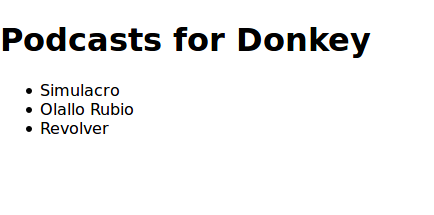
\includegraphics[scale=0.3]{react_first_app}
\end{figure}


\subparagraph{Firebase para aplicaciones web}

Para utilizar los servicios Firebase en una aplicación web
se siguen los mismos pasos que para el caso de 
aplicaciones para Android. Desde la consola de Firebase
se crea el proyecto y se obtiene un fragmento de código
de inicialización. Ese código  contiene información de inicialización para configurar el SDK de Firebase JavaScript a fin de usar Authentication, Cloud Storage, Realtime Database y Cloud Firestore.


Se puede acceder
a cada servicio desde el espacio de nombres de \sphinxcode{\sphinxupquote{firebase}}:
\begin{itemize}
\item {} 
\sphinxcode{\sphinxupquote{firebase.auth()}} - Authentication

\item {} 
\sphinxcode{\sphinxupquote{firebase.storage()}} - Cloud Storage

\item {} 
\sphinxcode{\sphinxupquote{firebase.database()}} - Realtime Database

\item {} 
\sphinxcode{\sphinxupquote{firebase.firestore()}} - Cloud Firestore

\end{itemize}

El proceso para usar el servicio de Realtime Database y Authentication
es el mismo que en Android. Los métodos de lectura y escritura
se mantienen cambiando únicamente la sintáxis.


\subparagraph{Firebase Realtime Database}
\label{\detokenize{firebase_web:firebase-realtime-database}}

Para leer la base de datos o escribir en ella, se necesita una instancia de
\sphinxcode{\sphinxupquote{firebase.database.Reference}}:

\fvset{hllines={, ,}}%
\begin{sphinxVerbatim}[commandchars=\\\{\}]
\PYG{o}{/}\PYG{o}{/} \PYG{n}{Obtiene} \PYG{n}{una} \PYG{n}{referecia} \PYG{n}{al} \PYG{n}{servicio} \PYG{n}{de} \PYG{n}{la} \PYG{n}{base} \PYG{n}{de} \PYG{n}{datos}
\PYG{n}{var} \PYG{n}{database} \PYG{o}{=} \PYG{n}{firebase}\PYG{o}{.}\PYG{n}{database}\PYG{p}{(}\PYG{p}{)}\PYG{p}{;}
\end{sphinxVerbatim}


\subparagraph{Lectura y escritura de datos.}
\label{\detokenize{firebase_web:lectura-y-escritura-de-datos}}
Para recuperar los datos de Firebase, se debe agregar un escuchador
asíncrono a \sphinxcode{\sphinxupquote{firebase.database.Reference}}. El escuchador se activa una vez para
el estado inicial de los datos y otra vez cuando los datos cambian.


Para ejecutar operaciones de escritura básicas, puedes usar \sphinxcode{\sphinxupquote{set()}} para guardar
datos en una referencia que especifiques y reemplazar los datos existentes en
esa ruta de acceso. Por ejemplo si se desea añadir un usuario a la base de datos,
una opción es la siguiente:

\fvset{hllines={, ,}}%
\begin{sphinxVerbatim}[commandchars=\\\{\}]
\PYG{n}{function} \PYG{n}{writeUserData}\PYG{p}{(}\PYG{n}{userId}\PYG{p}{,} \PYG{n}{name}\PYG{p}{,} \PYG{n}{email}\PYG{p}{,} \PYG{n}{imageUrl}\PYG{p}{)} \PYG{p}{\PYGZob{}}
\PYG{n}{firebase}\PYG{o}{.}\PYG{n}{database}\PYG{p}{(}\PYG{p}{)}\PYG{o}{.}\PYG{n}{ref}\PYG{p}{(}\PYG{l+s+s1}{\PYGZsq{}}\PYG{l+s+s1}{users/}\PYG{l+s+s1}{\PYGZsq{}} \PYG{o}{+} \PYG{n}{userId}\PYG{p}{)}\PYG{o}{.}\PYG{n}{set}\PYG{p}{(}\PYG{p}{\PYGZob{}}
    \PYG{n}{username}\PYG{p}{:} \PYG{n}{name}\PYG{p}{,}
    \PYG{n}{email}\PYG{p}{:} \PYG{n}{email}\PYG{p}{,}
    \PYG{n}{profile\PYGZus{}picture} \PYG{p}{:} \PYG{n}{imageUrl}
  \PYG{p}{\PYGZcb{}}\PYG{p}{)}\PYG{p}{;}
\PYG{p}{\PYGZcb{}}
\end{sphinxVerbatim}

\sphinxcode{\sphinxupquote{set()}} sobrescribe los datos en la ubicación que se especifíca, incluidos
los nodos secundarios.


\textbf{Detección de eventos en valores.}
\label{\detokenize{firebase_web:detecta-eventos-en-valores}}
Si deseas leer datos de una ruta de acceso y escuchar para detectar cambios,
usa los métodos \sphinxcode{\sphinxupquote{on()}} o \sphinxcode{\sphinxupquote{once()}} de \sphinxcode{\sphinxupquote{firebase.database.Reference}}
para observar eventos.

El evento más común es \sphinxcode{\sphinxupquote{value}} y permite leer una instantánea estática del
contenido de una ruta de acceso determinada, en el estado en que se encontraba
en el momento del evento. Este método se activa cuando se vincula el escuchador
y se vuelve a activar cada vez que cambian los datos (incluidos los de
nivel secundario). La devolución de llamada del evento recibe una instantánea
que contiene todos los datos de dicha ubicación, incluidos los datos
secundarios. Si no hay datos, la instantánea tiene un valor nulo.

En el siguiente ejemplo se muestra una aplicación donde se recupera el valor
de un recurso en la vase de datos:

\fvset{hllines={, ,}}%
\begin{sphinxVerbatim}[commandchars=\\\{\}]
\PYG{n}{var} \PYG{n}{resourceRef} \PYG{o}{=} \PYG{n}{firebase}\PYG{o}{.}\PYG{n}{database}\PYG{p}{(}\PYG{p}{)}\PYG{o}{.}\PYG{n}{ref}\PYG{p}{(}\PYG{l+s+s1}{\PYGZsq{}}\PYG{l+s+s1}{resource}\PYG{l+s+s1}{\PYGZsq{}}\PYG{p}{)}\PYG{p}{;}
\PYG{n}{resourceRef}\PYG{o}{.}\PYG{n}{on}\PYG{p}{(}\PYG{l+s+s1}{\PYGZsq{}}\PYG{l+s+s1}{value}\PYG{l+s+s1}{\PYGZsq{}}\PYG{p}{,} \PYG{n}{function}\PYG{p}{(}\PYG{n}{snapshot}\PYG{p}{)} \PYG{p}{\PYGZob{}}
  \PYG{n}{showValueOnScreen}\PYG{p}{(}\PYG{n}{snapshot}\PYG{o}{.}\PYG{n}{val}\PYG{p}{(}\PYG{p}{)}\PYG{p}{)}\PYG{p}{;}
\PYG{p}{\PYGZcb{}}\PYG{p}{)}\PYG{p}{;}
\end{sphinxVerbatim}

El escuchador recibe una \sphinxcode{\sphinxupquote{snapshot}} que contiene los datos de la ubicación
especifíca en la base de datos en el momento del evento. Se pueden recuperar
los datos de la \sphinxcode{\sphinxupquote{snapshot}} con el método \sphinxcode{\sphinxupquote{val()}}.


\textbf{Actualizar o borrar datos}
\label{\detokenize{firebase_web:actualizar-o-borrar-datos}}
Para escribir de forma simultánea en elementos secundarios específicos de un
nodo sin sobrescribir otros nodos secundarios, usa el método \sphinxcode{\sphinxupquote{update()}}.

También existe el método \sphinxcode{\sphinxupquote{push()}} para añadir una entrada con un identificador
único sobre una referencia.

La forma más sencilla de borrar datos es llamar a \sphinxcode{\sphinxupquote{remove()}} en una referencia a
la ubicación de los datos. Para borrar, también puedes especificar nulo como
el valor de otra operación de escritura, como \sphinxcode{\sphinxupquote{set()}} o \sphinxcode{\sphinxupquote{update()}}.


\paragraph{Firebase Authentication}

De este servicio se utilizó la autenticación con
correo electrónico y contraseña.
El SDK de Firebase Authentication proporciona métodos para crear y administrar usuarios que utilizan sus direcciones de correo electrónico y sus contraseñas para acceder.

Para crear una cuenta de usuario nueva se pasa la dirección de correo electrónico y la contraseña del nuevo usuario a \texttt{createUserWithEmailAndPassword} para crear la cuenta nueva.

\fvset{hllines={, ,}}%
\begin{sphinxVerbatim}[commandchars=\\\{\}]
\PYG{n}{firebase}\PYG{o}{.}\PYG{n}{auth}\PYG{p}{(}\PYG{p}{)}\PYG{o}{.}\PYG{n}{createUserWithEmailAndPassword}\PYG{p}{(}\PYG{n}{email}\PYG{p}{,} \PYG{n}{password}\PYG{p}{)}\PYG{o}{.}\PYG{n}{catch}\PYG{p}{(}\PYG{n}{function}\PYG{p}{(}\PYG{n}{error}\PYG{p}{)} \PYG{p}{\PYGZob{}}
  \PYG{o}{/}\PYG{o}{/} \PYG{n}{El} \PYG{n}{manejo} \PYG{n}{de} \PYG{n}{errores} \PYG{n}{va} \PYG{n}{aquí}
  \PYG{n}{var} \PYG{n}{errorCode} \PYG{o}{=} \PYG{n}{error}\PYG{o}{.}\PYG{n}{code}\PYG{p}{;}
  \PYG{n}{var} \PYG{n}{errorMessage} \PYG{o}{=} \PYG{n}{error}\PYG{o}{.}\PYG{n}{message}\PYG{p}{;}
\PYG{p}{\PYGZcb{}}\PYG{p}{)}\PYG{p}{;}
\end{sphinxVerbatim}


Cuando un usuario accede a tus apps, se pasan la dirección de correo electrónico y la contraseña al método \texttt{signInWithEmailAndPassword}.

\fvset{hllines={, ,}}%
\begin{sphinxVerbatim}[commandchars=\\\{\}]
\PYG{n}{firebase}\PYG{o}{.}\PYG{n}{auth}\PYG{p}{(}\PYG{p}{)}\PYG{o}{.}\PYG{n}{signInWithEmailAndPassword}\PYG{p}{(}\PYG{n}{email}\PYG{p}{,} \PYG{n}{password}\PYG{p}{)}\PYG{o}{.}\PYG{n}{catch}\PYG{p}{(}\PYG{n}{function}\PYG{p}{(}\PYG{n}{error}\PYG{p}{)} \PYG{p}{\PYGZob{}}
\PYG{o}{/}\PYG{o}{/} \PYG{n}{Aquí} \PYG{n}{se} \PYG{n}{manejan} \PYG{n}{los} \PYG{n}{errores}
\PYG{n}{var} \PYG{n}{errorCode} \PYG{o}{=} \PYG{n}{error}\PYG{o}{.}\PYG{n}{code}\PYG{p}{;}
\PYG{n}{var} \PYG{n}{errorMessage} \PYG{o}{=} \PYG{n}{error}\PYG{o}{.}\PYG{n}{message}\PYG{p}{;}
\PYG{o}{/}\PYG{o}{/} \PYG{o}{.}\PYG{o}{.}\PYG{o}{.}
\PYG{p}{\PYGZcb{}}\PYG{p}{)}\PYG{p}{;}
\end{sphinxVerbatim}

La manera recomendada de obtener el usuario actual es establecer un observador en el objeto \sphinxcode{\sphinxupquote{Auth}}:

\fvset{hllines={, ,}}%
\begin{sphinxVerbatim}[commandchars=\\\{\}]
\PYG{n}{firebase}\PYG{o}{.}\PYG{n}{auth}\PYG{p}{(}\PYG{p}{)}\PYG{o}{.}\PYG{n}{onAuthStateChanged}\PYG{p}{(}\PYG{n}{function}\PYG{p}{(}\PYG{n}{user}\PYG{p}{)} \PYG{p}{\PYGZob{}}
\PYG{k}{if} \PYG{p}{(}\PYG{n}{user}\PYG{p}{)} \PYG{p}{\PYGZob{}}
  \PYG{o}{/}\PYG{o}{/} \PYG{n}{El} \PYG{n}{usuario} \PYG{n}{ha} \PYG{n}{iniciado} \PYG{n}{sesión}
\PYG{p}{\PYGZcb{}} \PYG{k}{else} \PYG{p}{\PYGZob{}}
  \PYG{o}{/}\PYG{o}{/} \PYG{n}{No} \PYG{n}{hay} \PYG{n}{un} \PYG{n}{usuario} \PYG{n}{activo}
\PYG{p}{\PYGZcb{}}
\PYG{p}{\PYGZcb{}}\PYG{p}{)}\PYG{p}{;}
\end{sphinxVerbatim}

También se puede usar la propiedad \sphinxcode{\sphinxupquote{currentUser}} para obtener el usuario que
accedió. Si un usuario no accedió a su cuenta, \sphinxcode{\sphinxupquote{currentUser}} mostrará un
resultado nulo:

\fvset{hllines={, ,}}%
\begin{sphinxVerbatim}[commandchars=\\\{\}]
\PYG{n}{var} \PYG{n}{user} \PYG{o}{=} \PYG{n}{firebase}\PYG{o}{.}\PYG{n}{auth}\PYG{p}{(}\PYG{p}{)}\PYG{o}{.}\PYG{n}{currentUser}\PYG{p}{;}
\PYG{k}{if} \PYG{p}{(}\PYG{n}{user}\PYG{p}{)} \PYG{p}{\PYGZob{}}
  \PYG{o}{/}\PYG{o}{/} \PYG{n}{El} \PYG{n}{usuario} \PYG{n}{ha} \PYG{n}{iniciado} \PYG{n}{sesión}
\PYG{p}{\PYGZcb{}} \PYG{k}{else} \PYG{p}{\PYGZob{}}
  \PYG{o}{/}\PYG{o}{/} \PYG{n}{No} \PYG{n}{hay} \PYG{n}{un} \PYG{n}{usuario} \PYG{n}{activo}
\PYG{p}{\PYGZcb{}}
\end{sphinxVerbatim}


Para obtener la información del perfil de un usuario, puedes usar las propiedades de una instancia de \texttt{User}. Por ejemplo:

\fvset{hllines={, ,}}%
\begin{sphinxVerbatim}[commandchars=\\\{\}]
\PYG{n}{var} \PYG{n}{user} \PYG{o}{=} \PYG{n}{firebase}\PYG{o}{.}\PYG{n}{auth}\PYG{p}{(}\PYG{p}{)}\PYG{o}{.}\PYG{n}{currentUser}\PYG{p}{;}
\PYG{n}{var} \PYG{n}{name}\PYG{p}{,} \PYG{n}{email}\PYG{p}{,} \PYG{n}{photoUrl}\PYG{p}{,} \PYG{n}{uid}\PYG{p}{,} \PYG{n}{emailVerified}\PYG{p}{;}

\PYG{k}{if} \PYG{p}{(}\PYG{n}{user} \PYG{o}{!=} \PYG{n}{null}\PYG{p}{)} \PYG{p}{\PYGZob{}}
  \PYG{n}{name} \PYG{o}{=} \PYG{n}{user}\PYG{o}{.}\PYG{n}{displayName}\PYG{p}{;}
  \PYG{n}{email} \PYG{o}{=} \PYG{n}{user}\PYG{o}{.}\PYG{n}{email}\PYG{p}{;}
  \PYG{n}{photoUrl} \PYG{o}{=} \PYG{n}{user}\PYG{o}{.}\PYG{n}{photoURL}\PYG{p}{;}
  \PYG{n}{emailVerified} \PYG{o}{=} \PYG{n}{user}\PYG{o}{.}\PYG{n}{emailVerified}\PYG{p}{;}
  \PYG{n}{uid} \PYG{o}{=} \PYG{n}{user}\PYG{o}{.}\PYG{n}{uid}\PYG{p}{;}  \PYG{o}{/}\PYG{o}{/} \PYG{n}{El} \PYG{n+nb}{id} \PYG{k}{del} \PYG{n}{usuario} \PYG{n}{es} \PYG{n}{único} \PYG{n}{en} \PYG{n}{un} \PYG{n}{proyecto} \PYG{n}{de} \PYG{n}{Firebase}

\PYG{p}{\PYGZcb{}}
\end{sphinxVerbatim}


Para salir de la sesión de un usuario, se llama a \sphinxcode{\sphinxupquote{signOut}}:

\fvset{hllines={, ,}}%
\begin{sphinxVerbatim}[commandchars=\\\{\}]
\PYG{n}{firebase}\PYG{o}{.}\PYG{n}{auth}\PYG{p}{(}\PYG{p}{)}\PYG{o}{.}\PYG{n}{signOut}\PYG{p}{(}\PYG{p}{)}\PYG{o}{.}\PYG{n}{then}\PYG{p}{(}\PYG{n}{function}\PYG{p}{(}\PYG{p}{)} \PYG{p}{\PYGZob{}}
\PYG{o}{/}\PYG{o}{/} \PYG{n}{Se} \PYG{n}{cierra} \PYG{n}{la} \PYG{n}{sesión} \PYG{n}{exitosamente}
\PYG{p}{\PYGZcb{}}\PYG{p}{)}\PYG{o}{.}\PYG{n}{catch}\PYG{p}{(}\PYG{n}{function}\PYG{p}{(}\PYG{n}{error}\PYG{p}{)} \PYG{p}{\PYGZob{}}
  \PYG{o}{/}\PYG{o}{/} \PYG{n}{Un} \PYG{n}{error} \PYG{n}{ocurrió}
\PYG{p}{\PYGZcb{}}\PYG{p}{)}\PYG{p}{;}
\end{sphinxVerbatim}


\subparagraph{Firebase Hosting}
\label{\detokenize{firebase_web:firebase-hosting}}

Este servicio permite implementar y alojar los recursos estáticos de una aplicación
fácilmente (HTML, CSS, JavaScript, etc.). Todo el contenido se transmite a través
de HTTPS y está respaldado por una CDN global.

La ruta de implementación se muestra en las siguientes subsecciones.


\subparagraph{Instalar Firebase CLI.}
\label{\detokenize{firebase_web:instalar-firebase-cli}}
La CLI (interfaz de línea de comandos) de Firebase necesita Node.js y npm.

Para instalar Firebase CLI a través de npm se escribe los siguiente:

\fvset{hllines={, ,}}%
\begin{sphinxVerbatim}[commandchars=\\\{\}]
\PYG{n}{npm} \PYG{n}{install} \PYG{o}{\PYGZhy{}}\PYG{n}{g} \PYG{n}{firebase}\PYG{o}{\PYGZhy{}}\PYG{n}{tools}
\end{sphinxVerbatim}

Esto instala el comando \sphinxcode{\sphinxupquote{firebase}} de manera global.


\subparagraph{Inicializar la aplicación.}
\label{\detokenize{firebase_web:inicializar-la-aplicacion}}
Si se ejecuta el comando \sphinxcode{\sphinxupquote{firebase init}}, se crea un archivo de configuración
\sphinxcode{\sphinxupquote{firebase.json}} en la raíz del directorio del proyecto.


\subparagraph{Agregar un archivo.}
\label{\detokenize{firebase_web:agregar-un-archivo}}
Cuando se inicializa una aplicación, se pedirá proporcionar un directorio para
usarlo como raíz pública (el valor predeterminado es «public»). Si aún no
se tiene un archivo index.html válido en tu directorio raíz público, se creará
uno.


\subparagraph{Lanzar un sitio web.}
\label{\detokenize{firebase_web:implementar-un-sitio-web}}
Ejecutar \sphinxcode{\sphinxupquote{firebase deploy}} implementará la aplicación en el dominio
\sphinxcode{\sphinxupquote{\textless{}APP-DE-FIREBASE\textgreater{}.firebaseapp.com}}


\paragraph{Descripción de los componentes}
\label{\detokenize{code_docs:creacion-del-proyecto}}

La aplicación se creo utilizando la herramienta
\sphinxcode{\sphinxupquote{create-react-app}} y 
y después se le agregaron todos los servicios de Firebase
que se ocuparon. 

A partir de la estructura generada por \texttt{create-react-app}
todo el código fuente se agregó a la carpeta
\texttt{src}. Éste tiene la siguiente estructura:


\fvset{hllines={, ,}}%
\begin{sphinxVerbatim}[commandchars=\\\{\}]
src/
├── App.js
├── App.test.js
├── auth.js
├── components
│   ├── dashboard.js
│   ├── error\PYGZus{}msg.js
│   ├── landing\PYGZus{}page.js
│   ├── live\PYGZus{}image\PYGZus{}from\PYGZus{}robot.js
│   ├── log\PYGZus{}table.js
│   ├── navigation\PYGZus{}bar.js
│   ├── not\PYGZus{}found.js
│   ├── robot\PYGZus{}commands.js
│   ├── robot\PYGZus{}log.js
│   ├── robot\PYGZus{}selection.js
│   ├── robot\PYGZus{}status.js
│   ├── signin.js
│   ├── signout.js
│   ├── signup.js
│   ├── text\PYGZus{}to\PYGZus{}speech.js
│   ├── with\PYGZus{}authentication.js
│   └── with\PYGZus{}authorization.js
├── constants
│   └── routes.js
├── fire.js
├── index.css
├── index.js
└── registerServiceWorker.js
\end{sphinxVerbatim}


\subparagraph{App.js}
\label{\detokenize{code_docs:app-js}}
Se define el componente principal de la aplicación \texttt{App}, que se renderizará
al iniciarla. Se define el elemento \sphinxcode{\sphinxupquote{Router}} de React-Router
que define las rutas de los componentes que se renderizarán de acuerdo a lo
elegido por el usuario.


\subparagraph{auth.js}
\label{\detokenize{code_docs:auth-js}}
Aquí se definen las funciones para el inicio de sesión, registro de un usuario
y el cierre de sesión.


\subparagraph{fire.js}
\label{\detokenize{code_docs:fire-js}}
Aquí está la configuración de Firebase para usar los servicios de la base de datos
y de la autenticación.



\subparagraph{index.js}
\label{\detokenize{code_docs:index-js}}
En este archivo se llama al método render de \texttt{ReactDOM} para renderizar al
componente \sphinxcode{\sphinxupquote{App}}.


Dentro del directorio \texttt{components} están los archivos con los componentes de React para la aplicación.

\textbf{dashboard.js}
\label{\detokenize{code_docs:dashboard-js}}
Archivo con el componente \texttt{Dashboard} que muestra el panel de interacción con el robot.
Como estados define al usuario actual, un id y el nombre de un robot, el robot
que se selecciona en la lista de robots.

En el método \sphinxcode{\sphinxupquote{render()}} incluye otros componentes:
\texttt{LiveImage},
\texttt{RobotStatus},
\texttt{Robot\\Commands},
\texttt{TextToSpeech},
\texttt{RobotList} y
\texttt{RobotLogs}.


\textbf{error\_msg.js}
\label{\detokenize{code_docs:error-msg-js}}
Exporta al componente \texttt{ErrorMessage}, un mensaje de error utilizado en el SignUp y SignIn del usuario, pero puede
adaptarse a cualquier contexto pues simplemente recibe el texto del error
generado.

\textbf{landing\_page.js}
\label{\detokenize{code_docs:landing-page-js}}
Incluye a la subclase de \texttt{React.Component} \texttt{Landing} que se muestra al abrir la aplicación, estando o no una sesión
activa.


\textbf{live\_image\_from\_robot.js}
\label{\detokenize{code_docs:live-image-from-robot-js}}
Define al componente \texttt{LiveImage} que muestra la última imagen enviada por la cámara del robot. Tiene una imagen por
defecto, y espera una imagen codificada en base 64 obtendida desde Firebase.


\textbf{log\_table.js}
\label{\detokenize{code_docs:log-table-js}}
Se define \texttt{TableFromObject}, un componente que genera una tabla a partir de un JSON. Dos columnas lo
componen, en la primera están las llaves y en la segunda los valores de los
atributos del objeto de javascript. Se utiliza para mostrar los logs adquiridos
de Firebase.

\textbf{navigation\_bar.js}
\label{\detokenize{code_docs:navigation-bar-js}}
Hay tres componentes dentro de este archivo:
\texttt{NavigationAut}, el menú de navegación cuando el
usuario no ha iniciado sesión,
\texttt{NavigationNonAuth}, el menú cuando ha iniciado sesión y
\texttt{NavigationBar}, 
el que muestra al menú que corresponde al estado del usuario.


\textbf{robot\_commands.js}
\label{\detokenize{code_docs:robot-commands-js}}
Exporta el componente \texttt{RobotCommands} que es el control remoto del robot, aquí se envía información a la
de Firebase para que el robot realiza acciones como caminar, cambiar de postura,
o mover la cabeza, también se pueden actualizar algunos parámetros de caminado.

\textbf{robot\_log.js}
\label{\detokenize{code_docs:robot-log-js}}
Define a la clase \texttt{RobotLogs}, subclase de \texttt{React.Component}, que renderiza la tabla de logs con la información que se obtiene de
Firebase, también permite descargar el historial completo de logs para cada
robot.


\textbf{robot\_selection.js}
\label{\detokenize{code_docs:robot-selection-js}}
Se define al componente \texttt{RobotList} el cual maneja la selección de un robot y actualiza al
\sphinxcode{\sphinxupquote{Dashboard}} para que envíe a sus hijos el id del robot seleccionado.

\textbf{robot\_status.js}

Contiene al componente \texttt{RobotStatus} que muestra la batería y el estado de la conexión con el robot.

\textbf{signin.js}
\label{\detokenize{code_docs:signin-js}}
Se encuentra la clase \texttt{SignIn}, el componente que maneja el inicio de sesión de un usuario, utiliza al
objeto \sphinxcode{\sphinxupquote{auth}} para que el usuario utilice su dirección de correo y una
contraseña.


\textbf{signout.js}
\label{\detokenize{code_docs:signout-js}}
Define al componente \texttt{SignOutMenuItem} encargado de cerrar la sesión del usuario.


\textbf{signup.js}
\label{\detokenize{code_docs:signup-js}}
Contiene al componente \texttt{SignUp} en el que un nuevo usuario se registra. Utiliza las funciones
de autenticación de Firebase y además almacena al nuevo usuario a la base de
datos.

\textbf{text\_to\_speech.js}
\label{\detokenize{code_docs:text-to-speech-js}}
Define la clase \texttt{TextToSpeech}, el componente que envía una cadena de texto a Firebase para que el robot la
replique oralmente.

\subparagraph{constants/routes.js}
\label{\detokenize{code_docs:constants}}

Este archivo contiene las rutas de la aplicación.

\fvset{hllines={, ,}}%
\begin{sphinxVerbatim}[commandchars=\\\{\}]
\PYG{k+kr}{export} \PYG{k+kr}{const} \PYG{n+nx}{SIGN\PYGZus{}IN} \PYG{o}{=} \PYG{l+s+s1}{\PYGZsq{}/signin\PYGZsq{}}\PYG{p}{;}
\PYG{k+kr}{export} \PYG{k+kr}{const} \PYG{n+nx}{SIGN\PYGZus{}UP} \PYG{o}{=} \PYG{l+s+s1}{\PYGZsq{}/signup\PYGZsq{}}\PYG{p}{;}
\PYG{k+kr}{export} \PYG{k+kr}{const} \PYG{n+nx}{LANDING} \PYG{o}{=} \PYG{l+s+s1}{\PYGZsq{}/\PYGZsq{}}\PYG{p}{;}
\PYG{k+kr}{export} \PYG{k+kr}{const} \PYG{n+nx}{ROBOTS} \PYG{o}{=} \PYG{l+s+s1}{\PYGZsq{}/robots\PYGZsq{}}\PYG{p}{;}
\end{sphinxVerbatim}


La aplicación inicia mostrando el componente de la ruta \sphinxcode{\sphinxupquote{LANDING}}, que es
\sphinxcode{\sphinxupquote{Landing}}, el usuario selecciona \sphinxcode{\sphinxupquote{Sign In}} en el menú de navegación
se direcciona a la ruta \sphinxcode{\sphinxupquote{SIGN\_IN}}, si es un nuevo usuario puede dar click
en el botón que envía a la ruta \sphinxcode{\sphinxupquote{SIGN\_UP}}. Después de realzar un inicio de
sesión de cualquiera de las dos formas anteriores se redirecciona a la ruta
\sphinxcode{\sphinxupquote{ROBOTS}} que muestra al componente \sphinxcode{\sphinxupquote{Dashboard}}.

